\documentclass[a4paper, 10pt]{article}

\usepackage{tabularx} % extra features for tabular environment
\usepackage{amsmath}  % improve math presentation
\usepackage{graphicx} % takes care of graphic including machinery
\usepackage[margin=1in,letterpaper]{geometry} % decreases margins
\usepackage{cite} % takes care of citations
\usepackage[final]{hyperref} % adds hyper links inside the generated pdf file
\usepackage{ctex}
\usepackage{titlesec}
%\usepackage{CJKutf8, CJK}
\usepackage{makecell}                 % 三线表-竖线
\usepackage{booktabs}                 % 三线表-短细横线
% \usepackage{natbib}
\usepackage{graphicx}				  % 表格单元格逆时针
\usepackage{multirow}				  % 合并单元格
\usepackage{array}
\usepackage{amssymb}				  % 勾
\usepackage{amsmath}
\usepackage{longtable}                % 导入 longtable 宏包,表格自动换行
\usepackage{caption}
\usepackage{subcaption}               % 设置子图
\usepackage{color}					  % 文本颜色包
\usepackage{xcolor}
\usepackage{bbm}					  % 输入指示函数
\usepackage{tablefootnote}			  % 表格注释
\usepackage{pythonhighlight}
\usepackage{fancyhdr}
\usepackage{lastpage}
\pagestyle{fancy}
\fancyhf{}
\fancyhead{}
\fancyfoot{}
\fancyhead[R]{\small Page \thepage\ of \pageref*{LastPage}}
\fancyhead[L]{\zihao{-5} \songti 开题报告}

\usepackage{listings}                 % 导入代码块
\usepackage{xcolor}
\lstset{
	numbers=left, 
	tabsize=1,
	columns=flexible, 
	numberstyle=  \small, 
	keywordstyle= \color{ blue!70},
	commentstyle= \color{red!50!green!50!blue!50}, 
	frame=shadowbox, % 阴影效果
	rulesepcolor= \color{ red!20!green!20!blue!20} ,
	escapeinside=``, % 英文分号中可写入中文
	xleftmargin=2em,
	xrightmargin=2em, 
	aboveskip=1em,
} 

\hypersetup{
	colorlinks=true,       % false: boxed links; true: colored links
	linkcolor=blue,        % color of internal links
	citecolor=blue,        % color of links to bibliography
	filecolor=magenta,     % color of file links
	urlcolor=blue         
}
%++++++++++++++++++++++++++++++++++++++++
\titleformat{\section}{\Large\bfseries\songti}{\thesection}{1em}{}
\titleformat{\subsection}{\large\bfseries\songti}{\thesubsection}{1em}{}
\titleformat{\subsubsection}{\normalsize\bfseries\songti}{\thesubsubsection}{1em}{}
\titleformat{\paragraph}{\small\bfseries\songti}{\paragraph}{1em}{}
\titleformat{\subparagraph}{\footnotesize\bfseries\songti}{\subparagraph}{1em}{}

\begin{document}
	
	
	\title{\songti \zihao{4}开题报告}
	\author{\textrm{Ku Jui}}
	\date{\textrm{October 2023}}
	\maketitle
	
	\newpage
	
	\renewcommand{\figurename}{Figure} % 可以重新定义abstract,因为ctex会覆盖thebibliography
	% 	\begin{abstract}
		%		In this experiment we studied a very important physical effect by measuring the
		%		dependence of a quantity $V$ of the quantity $X$ for two different sample
		%		temperatures.  Our experimental measurements confirmed the quadratic dependence
		%		$V = kX^2$ predicted by Someone's first law. The value of the mystery parameter
		%		$k = 15.4\pm 0.5$~s was extracted from the fit. This value is
		%		not consistent with the theoretically predicted $k_{theory}=17.34$~s. We attribute %this
		%		discrepancy to low efficiency of our $V$-detector.
		%	\end{abstract}
	\renewcommand{\contentsname}{目录}
	\renewcommand{\tablename}{表}
	\renewcommand{\figurename}{图}
	\numberwithin{equation}{section}
	
	\tableofcontents  % 自动生成目录
	
	\newpage
	
	\part*{研究介绍}
	
	\section{研究意义}
	
	弱光图像增强(Low-light image enhancement, LLIE)是图像处理中的一个重要任务,其目标是提升在低光环境下拍摄的图像的感知质量。这个领域的近期进展主要由深度学习方法主导,包括不同的学习策略、网络架构、损失函数和训练数据。
	
	低光图像增强在不同领域享有广泛的应用,包括视觉监控、自动驾驶和计算摄影。特别是,智能手机摄影已经变得无处不在和突出。受限于相机光圈的大小、实时处理的要求以及存储器的约束,在昏暗环境中用智能手机的相机拍摄照片尤其具有挑战性。
	
	用于低光增强的传统方法包括基于直方图均衡的方法和基于 Retinex 模型的方法。然而,这些方法存在一些局限性,例如在 Retinex 模型中通常忽略噪声\cite{liu2021retinex, xu2020learning},因此在增强结果中保留或放大噪声;找到有效的先验或正则化是具有挑战性的,不准确的先验或正则化可能导致增强结果中的伪像和颜色偏差;由于其复杂的优化过程,运行时间相对较长。
	
	近年来基于深度学习的 LLIE 取得了引人注目的成功。基于深度学习的解决方案比传统方法具有更好的准确性、鲁棒性和速度,因此越来越受到关注。然而,现有的低光照图像增强技术聚焦于构建数据驱动的深度网络,通常其网络模型复杂,导致计算效率低、推理速度慢,并且由于对于训练数据分布的依赖性导致其在未知场景下的性能缺乏保障。
	
	为了解决这些问题并推动该领域的发展,研究者们提出了一些新颖的方法和工具。例如,他们提出了一个大尺度低光图像与视频数据集,并开发了一个包含多种主流 LLIE 方法的在线平台。这些工具可以帮助研究者和开发者更好地理解和改进现有技术,并为未来研究提供宝贵资源。
	
	\section{研究背景和现状}
	
	\subsection{传统低照度图像增强方法}
	\textbf{基于传统方法的低照度图像增强算法}通常利用单张图像自身的性质进行图像增强。主要包括灰度变换(GT)\textcolor{blue}{\cite{ueng1995gamma}}、直方图均衡化(HE)\textcolor{blue}{\cite{stark2000adaptive}}、Retinex模型\textcolor{blue}{\cite{land1971lightness}}、频域处理\textcolor{blue}{\cite{liu2021benchmarking}}、图像融合模型\textcolor{blue}{\cite{dai2019fractional}}、去雾模型\textcolor{blue}{\cite{ma2019improved}}等。在低照度图像增强的领域中,基于 Retinex 理论的方法非常受欢迎,并且吸引了众多研究者的关注。
	
	他们对这一模型进行了众多的优化和改进,显著提升了图像增强处理的效果。Retinex 理论,一种建立在实验和分析基础上的图像处理方法,通过将低照度图像分离成照度分量和反射分量,能够通过特定的处理技术来减弱或去除照度分量的影响,从而保留了物体的本质反射特性。然而,这种方法也有其不足之处。例如,仅使用反射分量作为增强结果可能会引起细节损失和颜色失真。
	
	\subsubsection{基于 Retinex 的方法}
	
	假设光照光滑,Retinex 理论通常将待处理图像 $z$ 看成反射图像 $m$ 和照度图像 $n$ 的合成. 其中, 反射分量包含图像中大量的本质内容; 照度分量则是包含光照等大量的外界信息, 决定图像的动态范围。Retinex 算法的核心思想是消除源图像照度分量干扰, 依据反射分量信息还原图像真实色彩。故 Retinex算法公式如式\ref{eq: Retinex model formula}所示。
	
	\begin{equation}
		\begin{aligned}
			z_i\left(x,y\right) = m_i\left(x,y\right) \cdot n_i\left(x,y\right)
		\end{aligned}
		\label{eq: Retinex model formula}
	\end{equation}
	
	其中$i \in \{R, G, B\}$,$m,n$ 是反射图像和照度图像,$(x,y)$为图像某像素的位置坐标。为了节省计算成本将式\ref{eq: Retinex model formula}变换至数域求解,如式\ref{eq: Retinex model formula log}所示。
	
	\begin{equation}
		\begin{aligned}
			\log z_i\left(x,y\right) = \log m_i\left(x,y\right) \cdot  \log n_i\left(x,y\right)
		\end{aligned}
		\label{eq: Retinex model formula log}
	\end{equation}
	
	令 $Z = \log z_i \left(x, y\right)$,$M = \log m_i \left(x, y\right)$,$N = \log n_i \left(x, y\right)$,则有 $M = Z - N$,将所得结果变换至指数域可得到图像反射分量,其算法处理过程如图\ref{fig: Retinex model}所示。
	
	\begin{figure}[htb]
		% read manual to see what [ht] means and for other possible options
		\centering 
		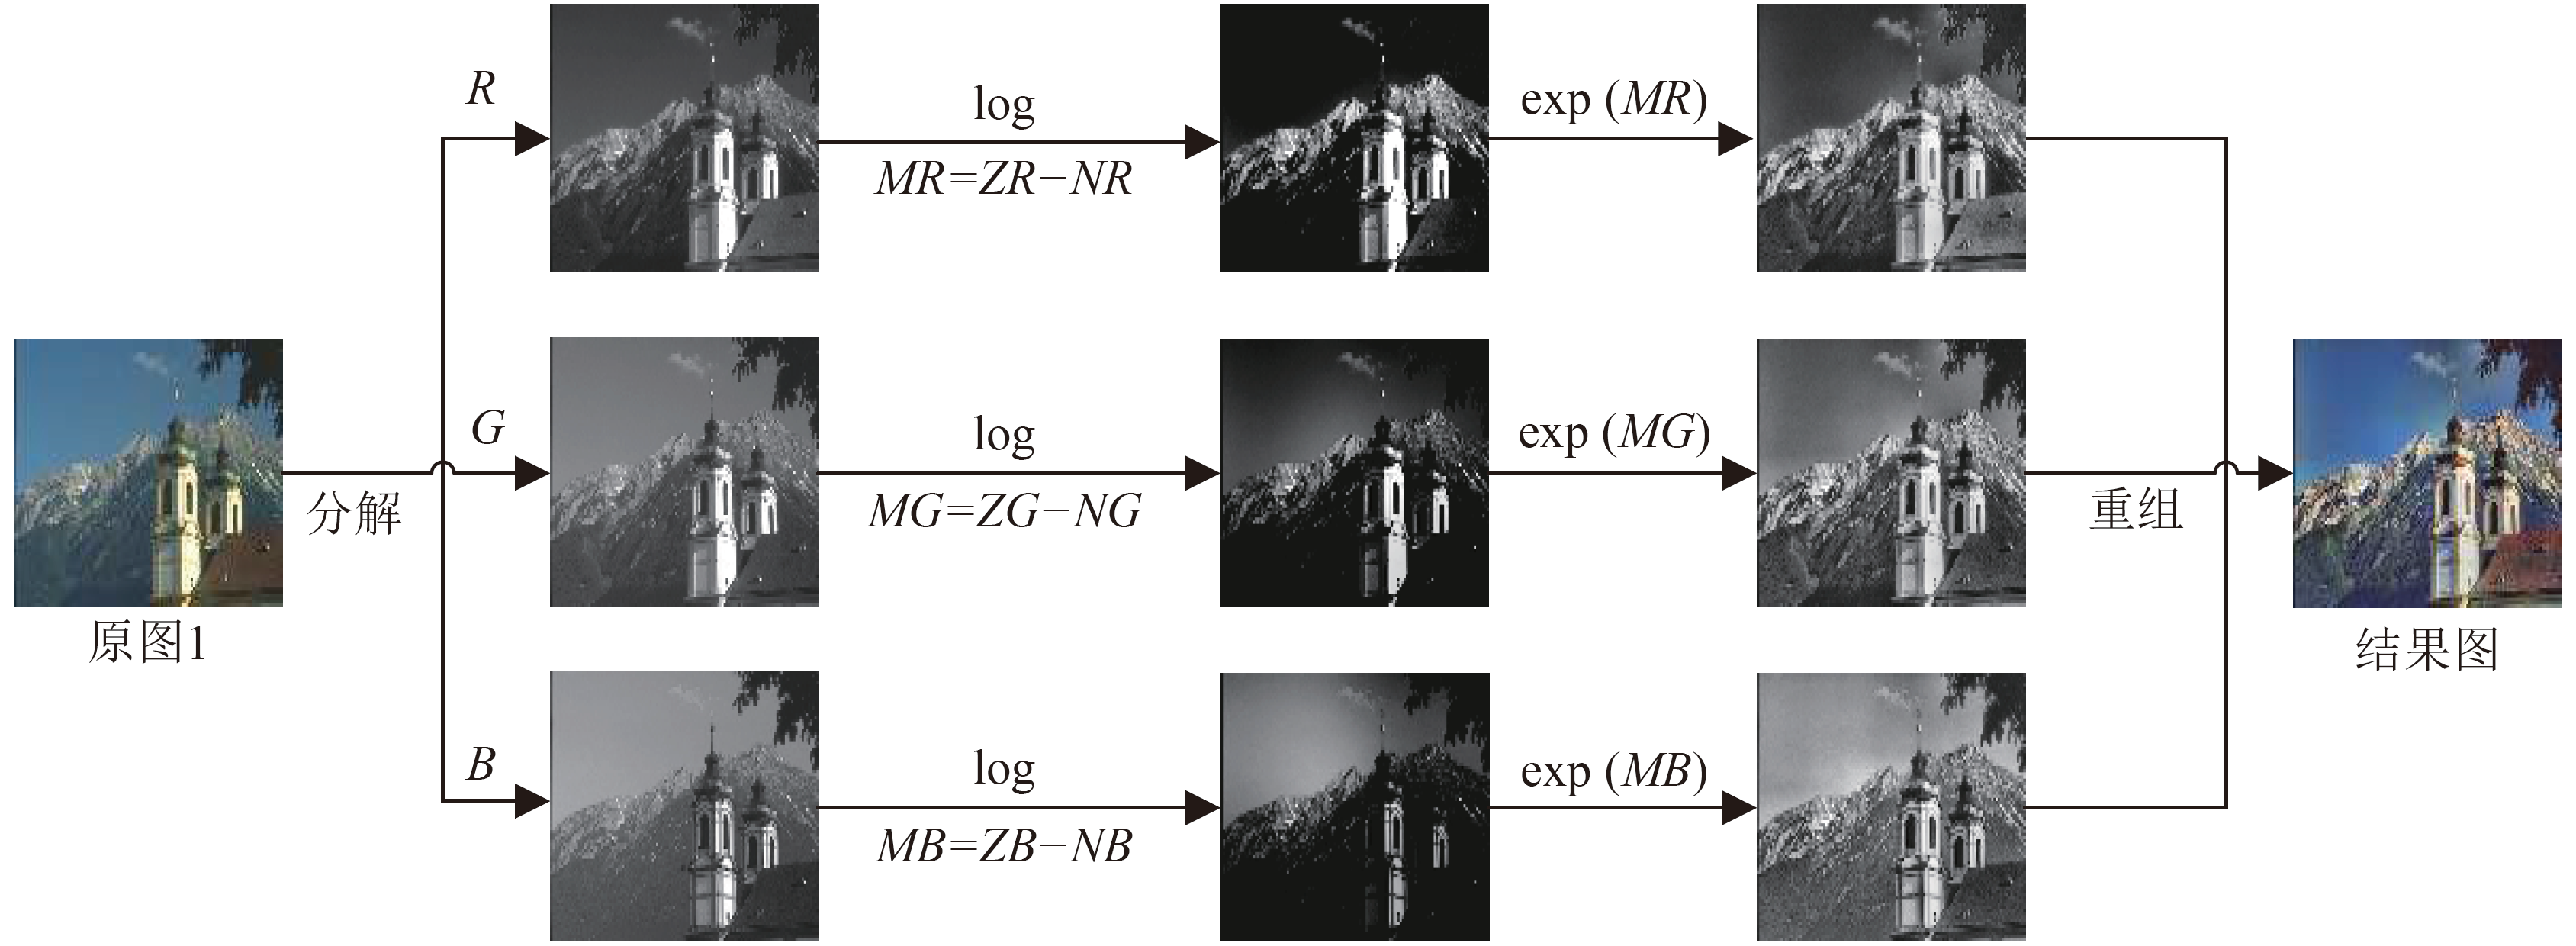
\includegraphics[width=\columnwidth]{picture/LLIE/Retinex Model/Retinex Model}
		%\captionsetup{font=scriptsize}
		\caption{
			\label{fig: Retinex model} 
			Retinex 算法处理过程
		}
	\end{figure}
	
	但是,传统 Retinex 算法能够很大程度改善图像质量,但在应用的过程中仍存在不可忽视的缺点。从图\ref{fig: Retinex Model}中可以看到基于传统 Retinex 算法的优势和局限性。由图\ref{fig: Retinex Model_Retinex}可见文献\cite{cooper2004analysis}算法能提高图\ref{fig: Retinex Model_input}的对比度和亮度, 整体颜色较清晰, 但天空部分的颜色并不自然, 并伴随伪影产生. 从图\ref{fig: Retinex Model_SSR}、图\ref{fig: Retinex Model_MSR}、图\ref{fig: Retinex Model_MSRCR}中明显看出, 基于中心/环绕的 Retinex 算法效果更有效. 但算法中参数选取具有局限性, 导致增强图像的对比度、色度、清晰度具有不确定性, 故增强效果并不理想。其中图\ref{fig: Retinex Model_SSR} SSR 算法能稍微改善天空的颜色, 但整体对比度有所下降, 且光晕现象较为严重; 图\ref{fig: Retinex Model_MSRCR} 中, MSRCR 算法因有颜色因子的缘故, 颜色明显要比图\ref{fig: Retinex Model_MSR} MSR 算法中图像的亮度和色度更为自然真实, 天空部分也少了许多伪影, 但改善效果仍不是最理想\cite{202013}。随着学者们对Retinex 算法的深入研究, 尤其针对传统Retinex 算法中的颜色失真和光晕现象这两大缺陷, 提出了大量的改进算法。
	
	\begin{figure}[htb] 
		\centering 
		\begin{subfigure}{0.18\textwidth}
			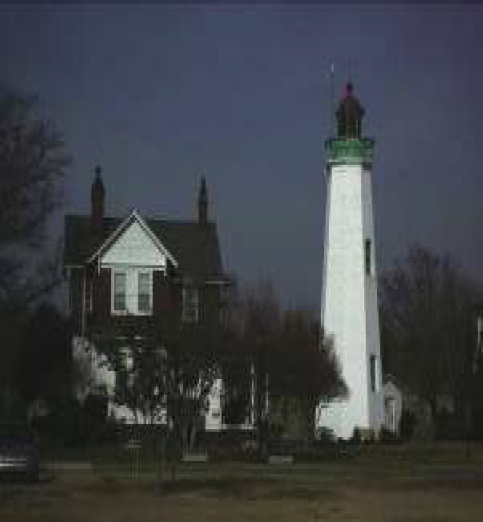
\includegraphics[width=\linewidth]{picture/LLIE/Retinex Model/input}
			\captionsetup{font=scriptsize}
			\caption{低照度图像}
			\label{fig: Retinex Model_input}
		\end{subfigure}
		\begin{subfigure}{0.18\textwidth}
			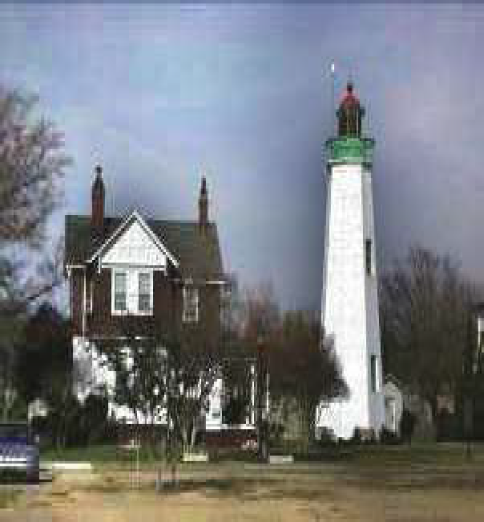
\includegraphics[width=\linewidth]{picture/LLIE/Retinex Model/Retinex}
			\captionsetup{font=scriptsize}
			\caption{Retinex\cite{cooper2004analysis}}
			\label{fig: Retinex Model_Retinex}
		\end{subfigure}
		\begin{subfigure}{0.18\textwidth}
			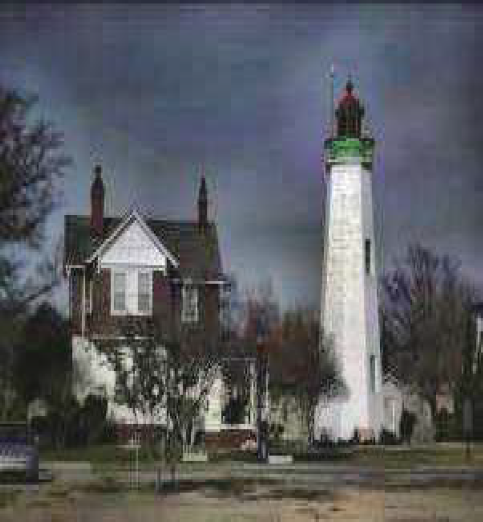
\includegraphics[width=\linewidth]{picture/LLIE/Retinex Model/SSR}
			\captionsetup{font=scriptsize}
			\caption{SSR}
			\label{fig: Retinex Model_SSR}	
		\end{subfigure}
		\begin{subfigure}{0.18\textwidth}
			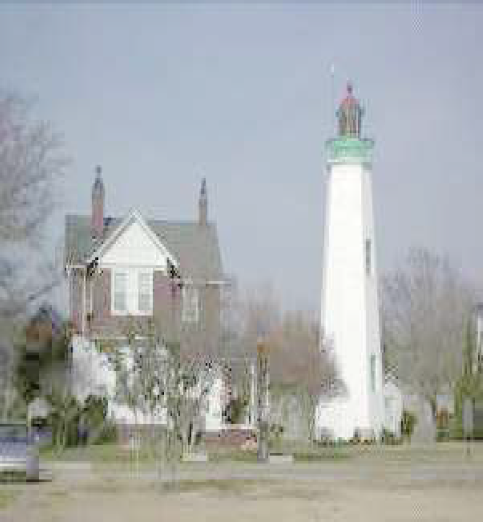
\includegraphics[width=\linewidth]{picture/LLIE/Retinex Model/MSR}
			\captionsetup{font=scriptsize}
			\caption{MSR}
			\label{fig: Retinex Model_MSR}	
		\end{subfigure}
		\begin{subfigure}{0.18\textwidth}
			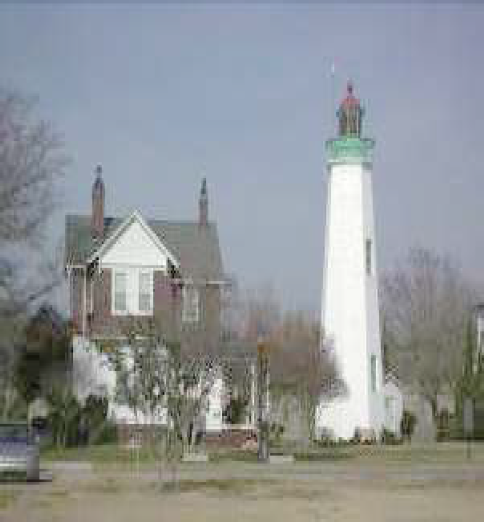
\includegraphics[width=\linewidth]{picture/LLIE/Retinex Model/MSRCR}
			\captionsetup{font=scriptsize}
			\caption{MSRCR}
			\label{fig: Retinex Model_MSRCR}	
		\end{subfigure}
		
		\captionsetup{font=scriptsize}
		\caption{
			\label{fig: Retinex Model}
			传统 Retinex 算法实验结果。
		}
	\end{figure}
	
	\subsubsection{基于直方图的方法}
	
	基于直方图的方法主要考虑直方图均衡化\cite{stark2000adaptive},通过对直方图\footnote{直方图统计图像每个灰度级的出现频率,其横坐标表示灰度级,纵坐标表示像素值为该灰度级下像素的频率。}的分布进行约束,改善图像的亮度分布。直方图描述了图像灰度级\footnote{图像灰度(image grayscale):把白色与黑色之间按对数关系分为若干等级,称为灰度。灰度分为256阶。用灰度表示的图像称作灰度图。}的分布情况,显示了图像的灰度范围和每个灰度级的出现频率。摄影师也常利用直方图判断整幅图像的明暗程度、对比度等图像特征,以便完成相应的后期处理。
	
	\begin{figure}[htb]
		% read manual to see what [ht] means and for other possible options
		\centering 
		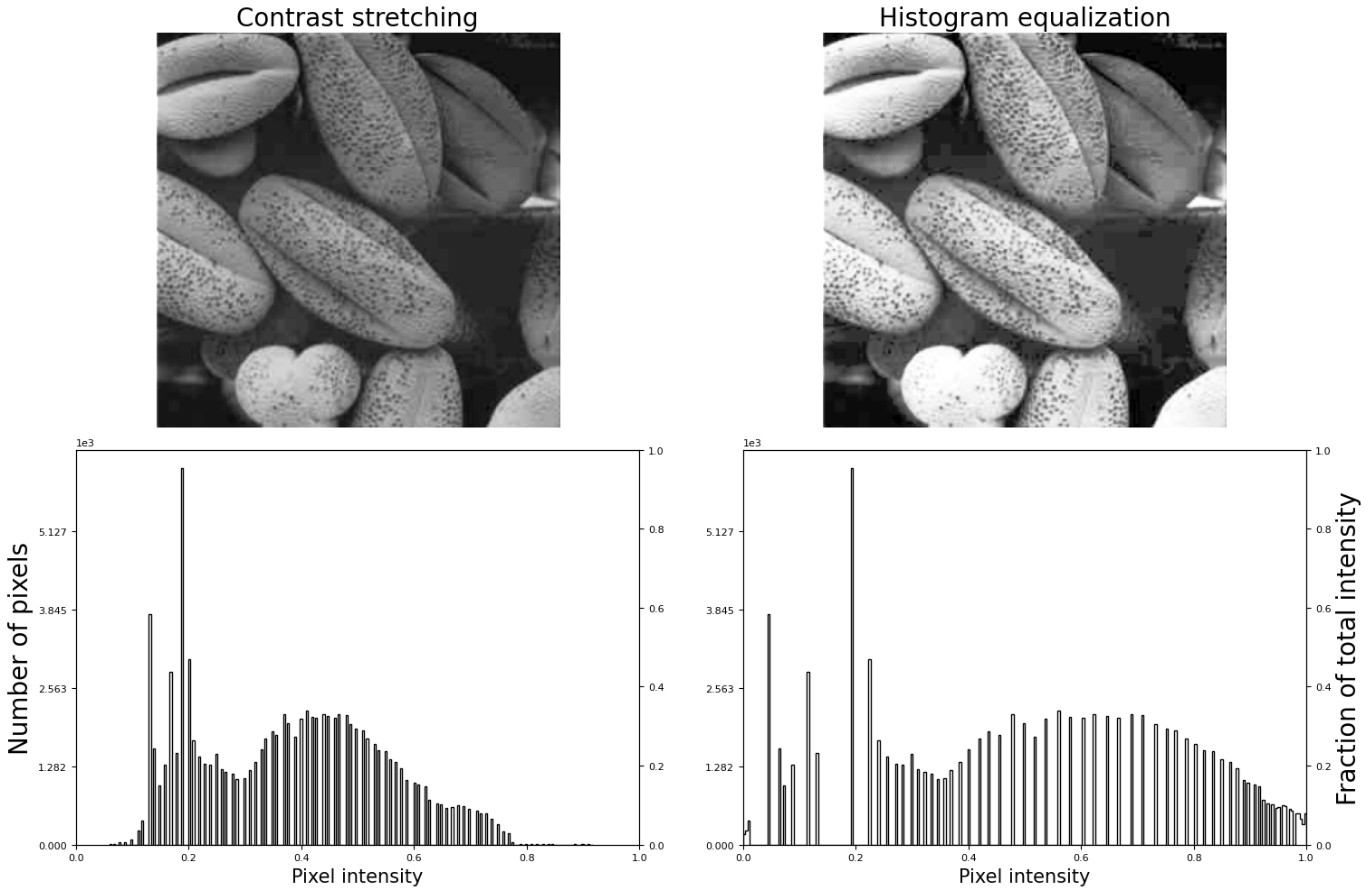
\includegraphics[width=\columnwidth]{picture/LLIE/HE/Histogram equalization}
		%\captionsetup{font=scriptsize}
		\caption{
			\label{fig: Histogram equalization} 
			直方图均衡化示意图
		}
	\end{figure}
	
	如图\ref{fig: Histogram equalization}所示,直方图均衡化重新调整图像的直方图分布,一方面增加了图像的全局对比度,另一方面使得亮度在整个图像的分布更加均匀。考虑一张包含L个灰度级的图像,其直方图可以表示为式\ref{eq: Histogram}
	\begin{equation}
		\begin{aligned}
			P(r_k) = \frac{n_k}{n}, k=0, 1, 2, \cdots, L-1
		\end{aligned}
		\label{eq: Histogram}
	\end{equation}
	其中, $r_k$ 表示第 $k$ 级灰度值,$n_k$表示图像中第 $k$ 级灰度值所对应的像素个数,$n$ 表示图像中的所有像素总数。显然,有 $\sum_{k} P(r_k)=1$。直方图均衡化是指存在一个变换函数 $s=T(r), 0 \leqslant r \leqslant 1$,能够将灰度级 $r$ 转化为灰度级 $s$。$T(r)$满足以下两个条件: 首先,$T(r)$ 在区间 $[0, 1]$ 上为单射函数且单调递增; 其次, $T(r) \in [0, 1]$ 。$T(r)$ 是单射函数保证了直方图均衡化存在反变换,而其单调递增的性质保证了变化后的图像与原图像之间存在保序性,以防变换后图像发生黑白颠倒。
	
	这样,一幅图像的灰度即视为 $[0,1]$ 上的随机变量,用 $p_r(r)$ 和 $p_s(s)$ 表示随机变量 $r$ 与 $s$的概率密度函数,那么,直方图均衡化即将 $T(r)$ 表示为式\ref{eq: HE}
	\begin{equation}
		\begin{aligned}
			s = T(r) = \int_{0}^{r} p_r(w) \mathrm{d}w
		\end{aligned}
		\label{eq: HE}
	\end{equation}
	可以证得,通过 $T(r)$ 的转化,有 $p_s(s) = 1$ ,即转换后的像素值在 $[0, 1]$ 上均匀分布。这时基于直方图变换的保序性,有 $$\int_{0}^{n} p_r(r) \mathrm{d}r = \int_{0}^{T(n)} p_s(s) \mathrm{d}s$$ 从而有: $$\frac{\mathrm{d}s}{\mathrm{d}r} = \frac{\mathrm{d}T(r)}{\mathrm{d}r} = p_r(r)$$ 代入上式,可得: $$p_s(s) = 1$$ 
	
	直方图均衡化的方法非常快速有效,并且是一个可逆操作,但缺点在于其不加选择地处理数据,可能增加背景噪声的对比度,同时降低有用的图像内容的对比度,导致视觉效果欠佳。此外,该方法也无法适用于复杂多变的低光照场景。
	
	\subsubsection{基于图像反相的方法}
	
	\begin{figure}[htbp] 
		% read manual to see what [ht] means and for other possible options
		\centering 
		% 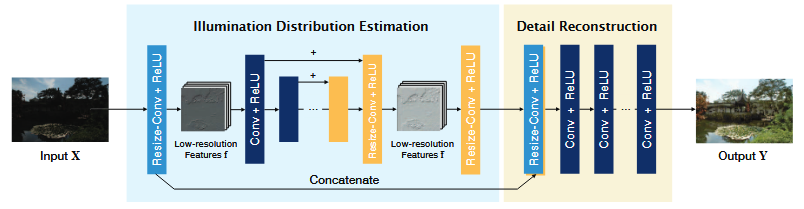
\includegraphics[width=0.8\columnwidth]{GLADNet}
		
		\begin{subfigure}{0.18\textwidth}
			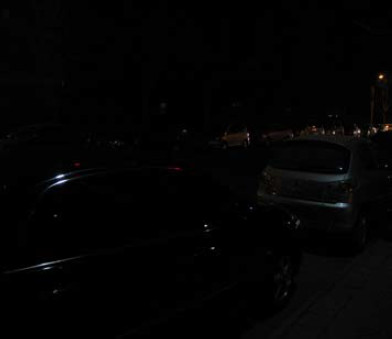
\includegraphics[width=\linewidth]{picture/LLIE/Inverse/LL input}
			\captionsetup{font=scriptsize}
			\label{fig: LL input}
		\end{subfigure}
		\begin{subfigure}{0.18\textwidth}
			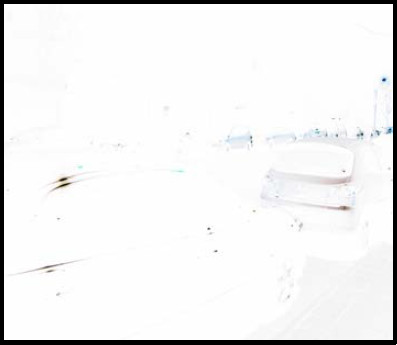
\includegraphics[width=\linewidth]{picture/LLIE/Inverse/Inversed}
			\captionsetup{font=scriptsize}
			\label{fig: Inversed}
		\end{subfigure}
		\begin{subfigure}{0.18\textwidth}
			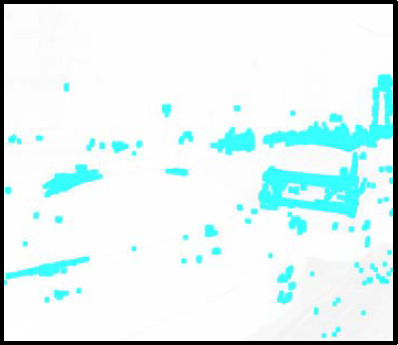
\includegraphics[width=\linewidth]{picture/LLIE/Inverse/marked image}
			\captionsetup{font=scriptsize}
			\label{fig: marked image}	
		\end{subfigure}
		\begin{subfigure}{0.18\textwidth}
			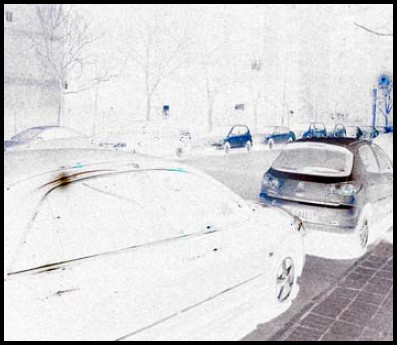
\includegraphics[width=\linewidth]{picture/LLIE/Inverse/de-haze}
			\captionsetup{font=scriptsize}
			\label{fig: de-haze}
		\end{subfigure}
		\begin{subfigure}{0.18\textwidth}
			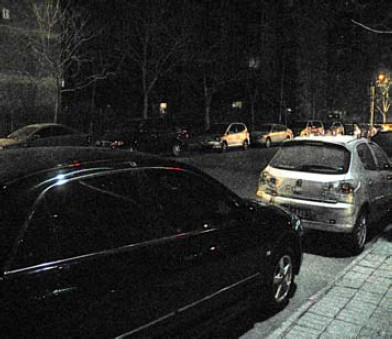
\includegraphics[width=\linewidth]{picture/LLIE/Inverse/Final output}
			\captionsetup{font=scriptsize}
			\label{fig: Final output}
		\end{subfigure}
%		\captionsetup{font=scriptsize}
		\caption{
			\label{fig: Image Inverse}
			(a) 低照度图片输入 I. (b) 从输入I获得的反向图片 R.(c) 标记图像:在至少一种颜色(RGB)通道中具有低强度的像素为绿色。 (d) 去雾: 使用公式获得输出 J. (e) 最终得输出结果 E.
		}
	\end{figure}
	
	基于图像反相的方法\cite{dong2010fast}利用低光照图像的反相\footnote{图像反相 (Image reverse phase) 就是图像的颜色色相反转。以前照相机的底片就是打印后的照片的反相。比如黑变白,蓝变黄、红变绿。对灰度级范围为 $[0 , L-1]$ 的一幅图像进行反转的操作为:$s = L - 1 - r$ 其中$r$和$s$分别代表处理前后的像素值。使用这种方式反转一幅图像的灰度级,可得到等效的照片底片。这种类型的处理特别适用于增强嵌入在一幅图像的暗区域中的白色和灰色细节,特别是当黑色面积在尺寸上占主导地位时}与有雾图像的相似性,通过对低光照图像反相进行去雾后再次进行反相,得到最终的低光照增强效果。在图像反相中,对于动态范围为 $[ 0, 255]$ 的图像,其反相图像 $\mathbf{R}$ 为式\ref{eq: Image Reverse} 
	
	\begin{equation}
		\begin{aligned}
			\mathbf{R}^c (x) = 255 - \mathbf{I}^c(x)
		\end{aligned}
		\label{eq: Image Reverse}
	\end{equation}
	
	其中,$c$ 为 \textbf{RGB} 颜色通道。大多数有雾图像符合暗通道先验,其特点是对于背景及天空等区域,\textbf{RGB} 3个通道的像素值都很高,而其他区域至少有一个通道的像素值较低,作者发现低光照图像的反相也具有同样特点。如图\ref{fig: Image Inverse}所示。
	
	基于图像反相的方法虽然运算速度很快,但需要基于低光照图像反相与有雾图像相似这一前提,而改前提始终是统计意义上的,无法得出二者之间更本质的联系,因而限制了这一方法的继续发展。由于没有考虑低光照图像的结构信息,因此该类方法还常常导致增强结构出现明显的黑边。
	
	\subsection{基于深度学习的低照度图像增强方法}
	
	从 2017 年 LLNet\cite{lore2017llnet}的出现,基于深度学习的低照度图像增强方法受到广泛关注,截至 2023 年已经出现了上百种基于深度学习的低照度图像增强方法,这充分反映了基于深度学习的方法具有更好的准确性、鲁棒性和更快的速度。
	
	基于深度学习的低照度图像增强算法,根据其学习和训练方式又分为四类,分别为有监督学习、无监督学习、半监督学习和零采样(Zero-shot)学习方法\cite{tang2023low}。
	
	\subsubsection{有监督学习}
	
	有监督学习最重要的特定是需要标记的数据集,监督学习是从标记的训练数据中学习模型,然后使用模型来训练一些新数据的标签。同时,预测标签与给点标签越相似,监督学习算法越好。基于监督学习的低照度图像增强方法大致可分为端到端 (End-to-end) 方法和 Retinex 理论方法。
	
	\paragraph{端到端 (End-to-end) 方法}
	
	\begin{figure}[htbp] 
		% read manual to see what [ht] means and for other possible options
		\centering 
		% 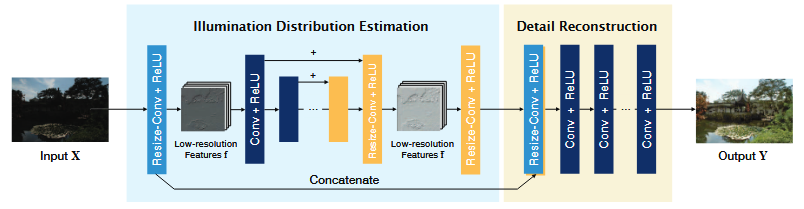
\includegraphics[width=0.8\columnwidth]{GLADNet}
		
		\begin{subfigure}{0.45\textwidth}
			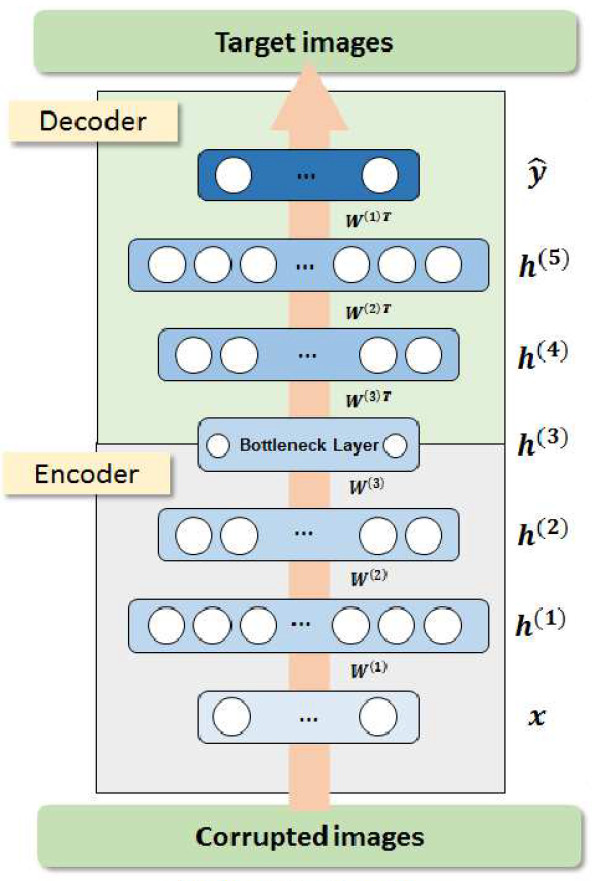
\includegraphics[width=\linewidth]{picture/LLIE/LLNet/Module Structure}
			\captionsetup{font=scriptsize}
			\caption{Module Structure}
			\label{fig: Module Structure}
		\end{subfigure}
		\begin{subfigure}{0.18\textwidth}
			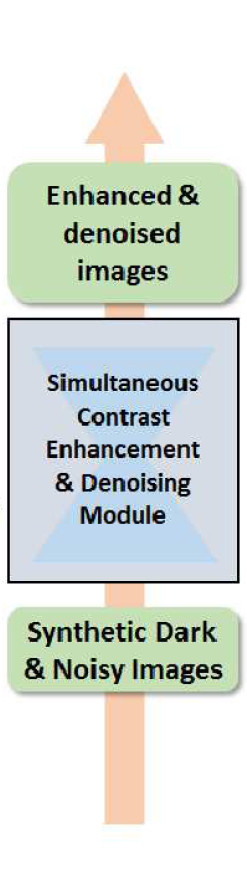
\includegraphics[width=\linewidth]{picture/LLIE/LLNet/LLNet}
			\captionsetup{font=scriptsize}
			\caption{LLNet}
			\label{fig: LLNet}
		\end{subfigure}
		\begin{subfigure}{0.175\textwidth}
			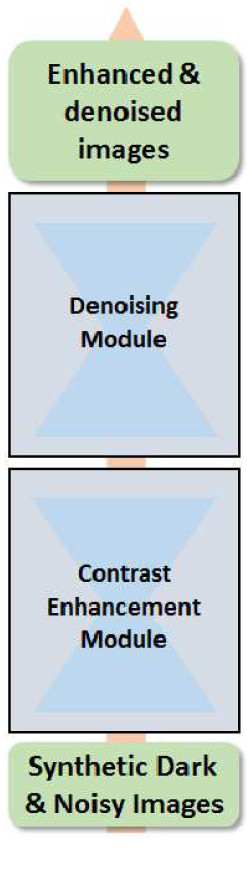
\includegraphics[width=\linewidth]{picture/LLIE/LLNet/S-LLNet}
			\captionsetup{font=scriptsize}
			\caption{S-LLNet}
			\label{fig: S-LLNet}	
		\end{subfigure}
		\captionsetup{font=scriptsize}
		\caption{
			\label{fig: LLNet Architecture}
			LLNet结构示意图
		}
	\end{figure}
	
	\textbf{LLNet}\cite{lore2017llnet}是早期提出的一种基于深度学习的方法,它利用一种特殊的堆叠稀疏去噪自编码器从低光照图像中提取特征,并进行自适应增强与去噪。接着,Lv等人\cite{lv2018mbllen}介绍了 \textbf{MBLLEN},这是一个包含特征提取模块(FEM)、增强模块(EM)和融合模块(FM)的多分支图像增强网络。MBLLEN通过多层次的特征提取和多子网络的增强处理,最终通过融合模块产生增强后的图像,有效地减少低照度区域的噪声和伪影。
	
	\begin{figure}[htb]
		% read manual to see what [ht] means and for other possible options
		\centering 
		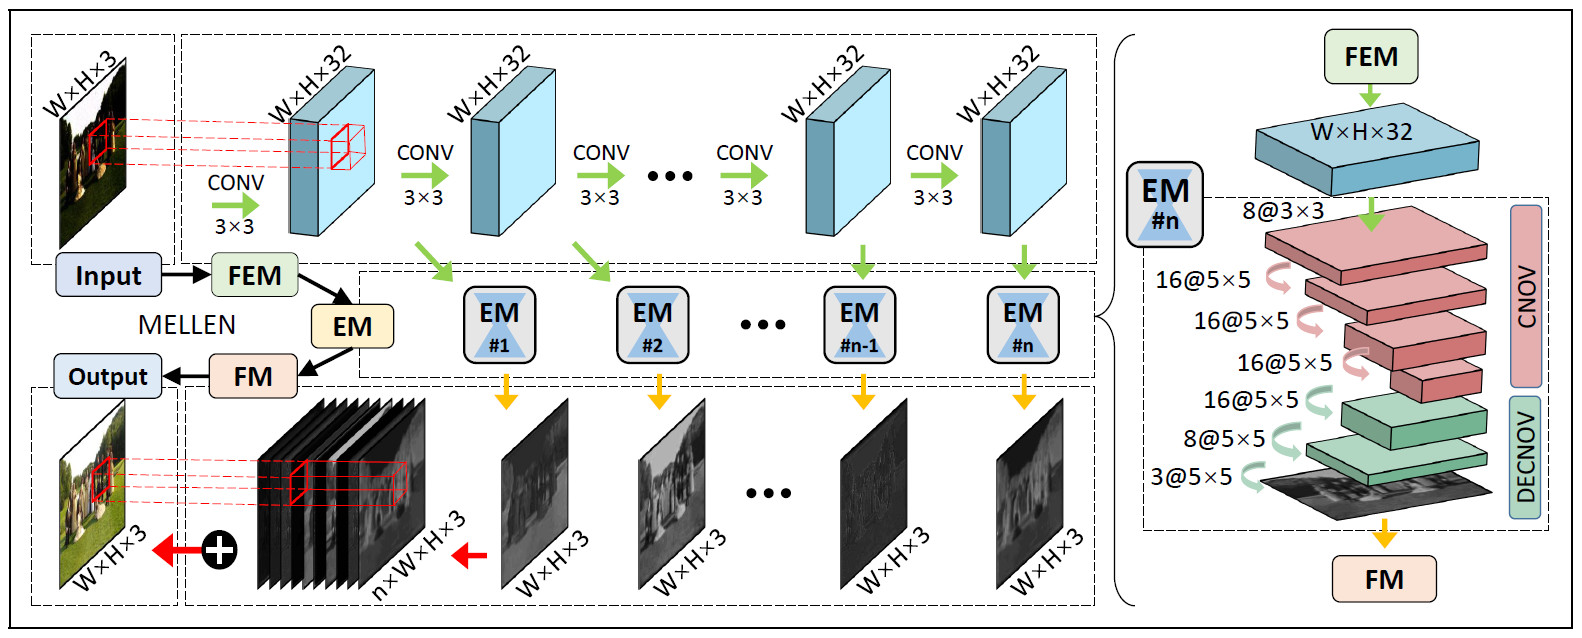
\includegraphics[width=\columnwidth]{picture/LLIE/MBLLEN/MBLLEN Architecture}
		%\captionsetup{font=scriptsize}
		\caption{
			\label{fig: MBLLEN Architecture} 
			MBLLEN 结构图。
		}
	\end{figure}
	
	此外,Wang 等人\cite{wang2018gladnet}提出的 \textbf{GLADNet} 网络使用编码器-解码器架构处理输入图像,生成全局照度估计,并在此基础上进行图像重构。该网络的有效性通过Google Cloud Vision API2上的目标识别测试得到了验证。\textbf{TBEFN}\cite{lu2020tbefn}是一种多曝光融合网络,通过两个子网络生成增强图像,进而通过平均融合法降低噪声,并对效果进行细化。\textbf{PRIEN}\cite{li2021low}是一种使用递归层和残差块的递归单元的渐进式增强网络,它直接将低照度图像输入到双注意模型中提取特征,并通过递归处理减少参数数量,尽管网络结构简单,但增强效果显著。最后,\textbf{C-LIENet}\cite{ravirathinam2021c}包含一个由卷积层构成的编码器-解码器结构,并通过其独特的多上下文特征提取模块层级提取特征,该方法采用了一种三部分的损失函数,有效地处理局部特征、结构相似性和细节性。另外,Lim等人\cite{lim2020dslr}提出的深度拉普拉斯复原器(\textbf{DSLR})能够调整输入图像的全局亮度和局部细节,并通过多尺度拉普拉斯残差块在特征空间中增强连接,提高了训练的效率。
	
	\paragraph{Retinex 理论方法}
	
	\begin{figure}[htb]
		% read manual to see what [ht] means and for other possible options
		\centering 
		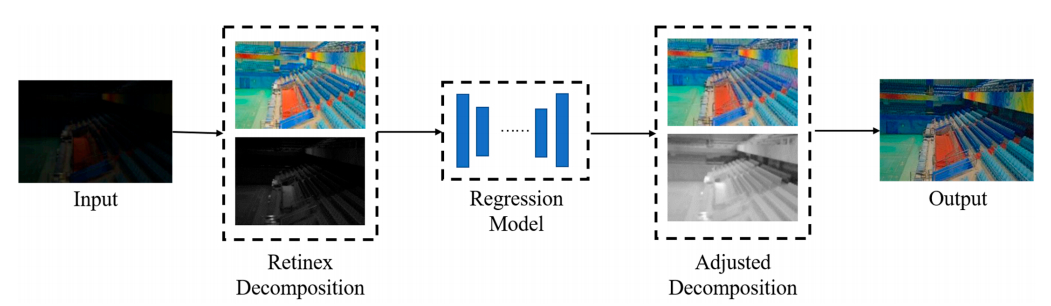
\includegraphics[width=0.7\columnwidth]{picture/LLIE/RetinexNet/RetinexNet}
		%\captionsetup{font=scriptsize}
		\caption{
			\label{fig: RetinexNet} 
			RetinexNet算法结构图。主要由三个部分组成,分解(Decomposition),调节(Adjustment)和重构(Reconstruction)。
		}
	\end{figure}
	
	相较于传统的端到端网络学习方法,融合深度学习与 Retinex 理论的策略在某些情况下展现出了更优越的图像增强性能。Wei等人\cite{wei2018deep}率先结合数据驱动方法与 Retinex 理论,开发出了一种深度学习框架 \textbf{RetinexNet}。这个框架通过分解网络将图像拆分为反射率图和结构感知的照明图,随后利用增强网络对大范围的照明区域进行优化。图像的最终效果通过局部裁剪和 BM3D 去噪技术得到提升。Liang等人\cite{shen2017msr}对MSR(多尺度Retinex)理论进行了深入的探究,并提出了 \textbf{MSR-net},它包含了多尺度对数变换、卷积差分和颜色恢复等三个模块。这个网络通过学习由 Photoshop 调整的合成低照度图像对,实现了从低照度到真实图像的直接端到端映射。\textbf{KinD}\cite{zhang2019kindling}则基于 Retinex 理论构建了一个分为照明调节和退化去除两个分支的深度网络。该网络包括层分解、反射率恢复和照度调整三个模块,并通过多尺度照度增强模块来减少增强图像的噪声和失真。
	
	\paragraph{基于 Transformer 的方法}
	
	当前,以 Vision Transformer(ViT) 为核心的监督学习任务受到广泛关注。在这一领域中,Cui等人\cite{cui2022illumination}开发了一种名为照明自适应变压器 (Illumination-Adaptive Transformer, \textbf{IAT}) 的网络。这个网络是全监督训练模式下的超轻量级架构。它借鉴了目标检测网络 \textbf{DETR} (Detection Transformer)的设计理念\cite{carion2020end},实现了一个端到端的变压器结构,有效地解决了低照度环境下的视觉效果问题。IAT网络的主要优点在于其出色的性能和快速的处理速度。另一方面,Wang等人\cite{wang2023ultra}提出了一种新型的低照度变压器网络,名为\textbf{LLFormer}。LLFormer的关键特性是其基于轴的多头自注意力和跨层注意力融合块,这大大减少了计算的复杂度。此外,Wang等人还创建了一个4K和8K超高清图像(UHD-LOL)的基准数据集,用以评估LLFormer的性能。这代表了首次尝试解决超高清低照度图像增强(UHD-LLIE)的任务。
	
	\subsubsection{无监督学习}
	
	尽管有监督学习方法在图像增强中取得了一定的成效,但它面临着两大主要限制。首先,可用于训练的成对图像数据集是有限的。其次,在这样的成对数据集上训练的模型容易出现过拟合的问题。为了克服这些挑战,研究者们转向了无监督学习方法。无监督学习的主要特点是在没有标签数据的情况下进行学习。Jiang等人\cite{jiang2021enlightengan}开创性地提出了一种名为 \textbf{EnlightenGAN} 的无监督学习方法。这是首个在该领域成功应用非配对训练的例子。EnlightenGAN的主要创新在于两个方面:一是其全局-局部判别器结构,用于处理输入图像中的空间光照变化;二是结合自特征保留损失和自正则化注意力机制,确保增强后图像的内容特征保持不变。此外,Fu等人\cite{fu2022gan}设计了一种名为 \textbf{LE-GAN} 的低照度增强网络,使用不变身份损失和注意力模块来提升图像特征提取,同时实现降噪和细节增强。该网络通过不变身份损失解决过度曝光的问题。他们还构建并公开了一个较大的非配对低照度/正常照度图像数据集PNLI。
	
	\begin{figure}[htb]
		% read manual to see what [ht] means and for other possible options
		\centering 
		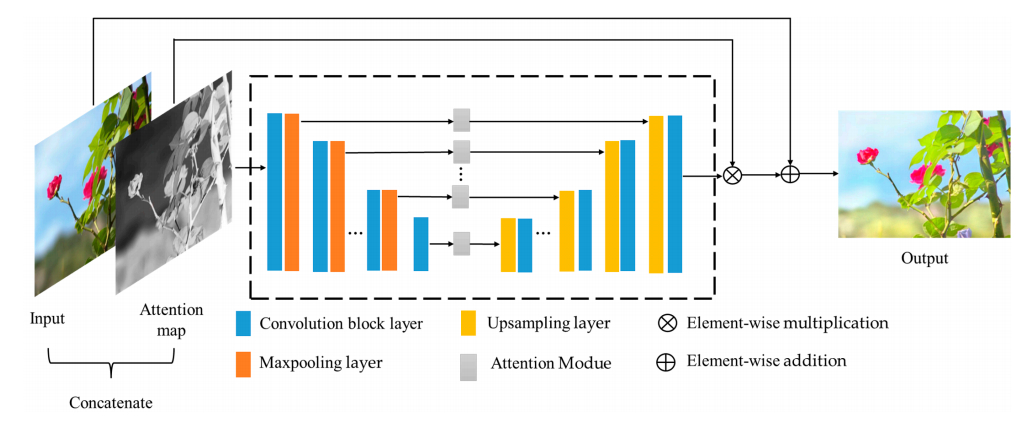
\includegraphics[width=0.7\columnwidth]{picture/LLIE/EnlightenGAN/EnlightenGAN}
		%\captionsetup{font=scriptsize}
		\caption{
			\label{fig: EnlightenGAN} 
			EnlightenGAN 结构图
		}
	\end{figure}
	
	Ni等人\cite{ni2020towards}提出了 \textbf{UE-GAN},一种基于单个深度GAN并结合注意力机制的无监督增强方法。UE-GAN 通过引入保真度损失和质量损失来处理无监督图像增强,确保增强后的图像在内容上与输入图像保持一致。Zhang等人\cite{zhang2021unsupervised}则提出了一种基于直方图均衡化的无监督低照度图像增强方法 \textbf{HEP}。该方法采用噪声分离模块(NDM),对非配对图像对的反射率图中的噪声和内容进行分离,并通过直方图均衡化和噪声分离模块有效增强图像的纹理信息和亮度细节,同时抑制图像暗黄色区域的噪声。
	
	\subsubsection{半监督学习}
	
	近年来,半监督学习作为一种新兴的学习方法,结合了监督学习的精确性和非监督学习的广泛适用性。这种学习方法既利用了有标签的数据,也依赖于无标签的数据。其显著特点是能够在有限的标记样本和大量未标记样本的情况下训练有效的分类器,从而解决在标记样本稀缺、未标记样本丰富的情境下的学习问题。
	
	\begin{figure}[htb]
		% read manual to see what [ht] means and for other possible options
		\centering 
		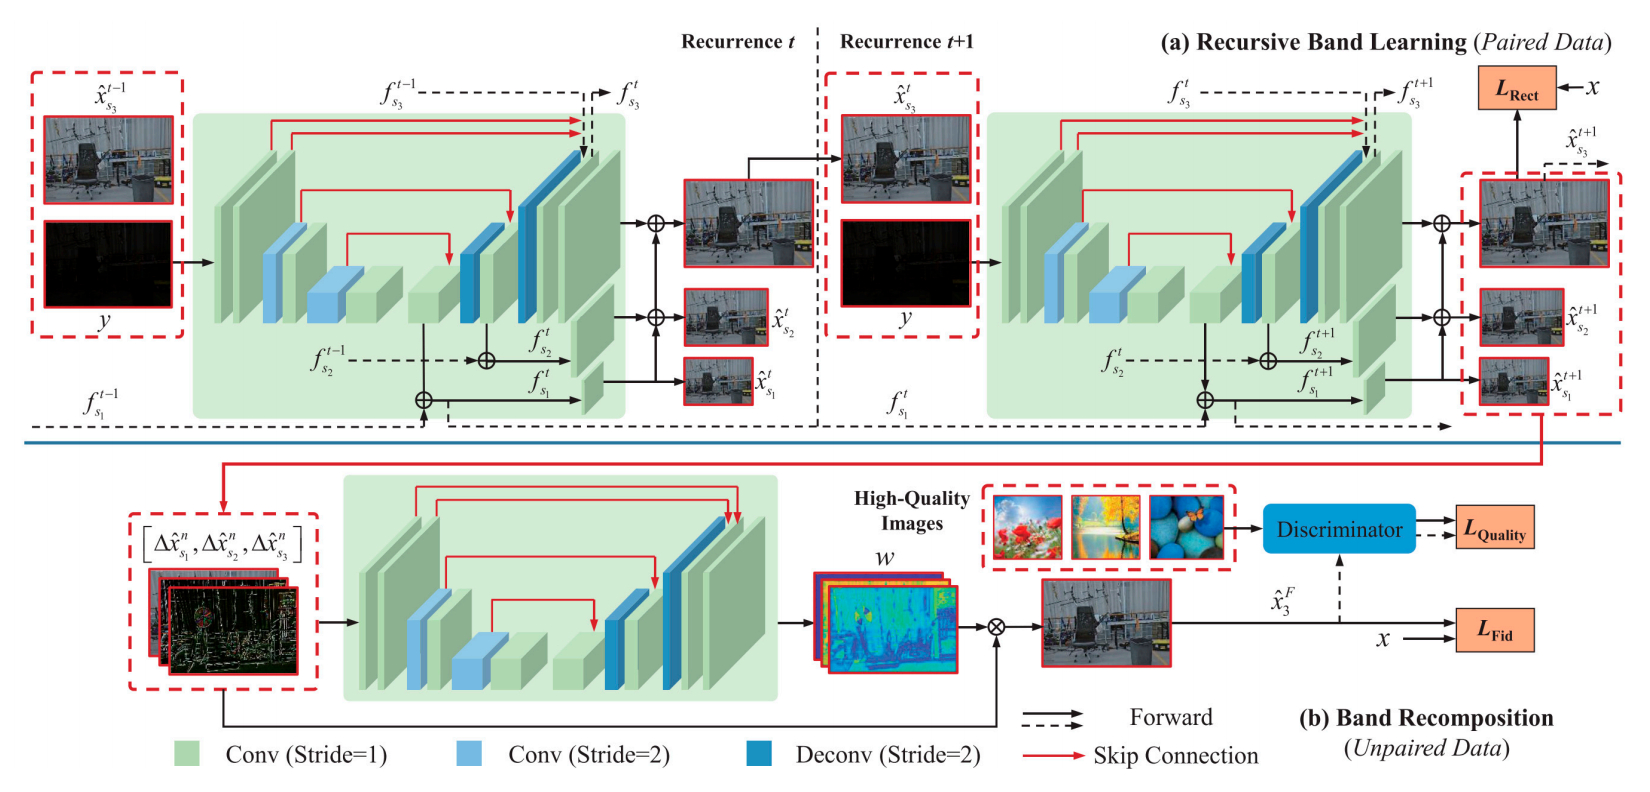
\includegraphics[width=0.7\columnwidth]{picture/LLIE/DRBN/DRBN}
		%\captionsetup{font=scriptsize}
		\caption{
			\label{fig: DRBN} 
			DRBN 结构图
		}
	\end{figure}
	
	在这一领域中,Yang等人\cite{qiao2021deep}提出了一种名为 \textbf{DRBN} 的半监督低照度图像增强方法,该方法基于频带表示。DRBN是一种深度递归频带网络,它通过对低光照/标准光照图像对的频带表示进行线性恢复,然后对这些频带进行重新定位,以改善频带表示。这种方法不仅有效地去除了图像噪声,还能优化图像细节。另一方面,Robert等人开发了一种名为 \textbf{HybirdNet} 的半监督学习网络\cite{robert2018hybridnet}。该网络分为两个分支:第一个分支接收监督信号并专注于提取不变的成分,而第二个分支完全无监督,其目的是重建第一个分支丢弃的模型信息,作为输入数据的补充。
	
	\subsubsection{Zero-Shot 学习}
	
	Zero-shot 学习的一个显著优点是它无需依赖预先训练的数据集。这种方法允许直接将待处理的低光照图像作为输入,而无需经过预先的训练阶段。在这一方法论下,Zhu等人\cite{zhu2020zero}提出了一种创新的三分支全卷积神经网络,名为\textbf{RRDNet}。该网络将输入图像拆分为三个组成部分:光照、反射和噪声。通过特殊设计的迭代损失函数,网络能够对噪声进行精确估计并有效恢复光照部分,实现清晰的噪声预测,进而成功去除图像中的噪声。RRDNet还引入了一种新型的损失算法,该算法依据图像的亮度分布来估计暗区的噪声,避免了暗区噪声的过度放大。受到超分辨率模型的启发,Zhang等人\cite{zhang2019zero}开发了一种专门用于实时测试的CNN网络\textbf{ExCNet}。在实际应用中,ExCNet能够估计出最适合当前背光图像的参数曲线,这使得网络非常适合在复杂拍摄环境和恶劣的背光条件下进行图像增强。ExCNet的一个独特优势是其能够利用前一帧的参数作为参考,从而在视频增强过程中避免产生伪影。
	
	\begin{figure}[htb]
		% read manual to see what [ht] means and for other possible options
		\centering 
		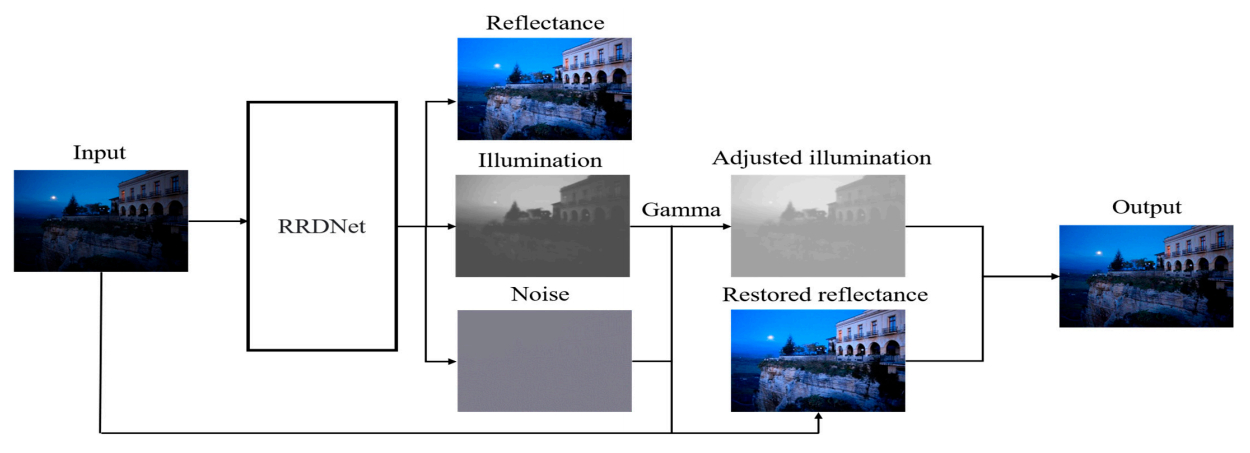
\includegraphics[width=0.7\columnwidth]{picture/LLIE/RRDNet/RRDNet}
		\caption{
			\label{fig: RRDNet} 
			RRDNet 结构图
		}
	\end{figure}
	
	\subsection{研究目的}
	
	现有的方法仍有很大的改进空间,例如如何在提高亮度的同时消除产生的噪声,如何避免颜色失真现象等。一些现有的方法可以有效地解决一个问题,但往往会忽略了其他问题。不同的方法在不同的数据集上往往具有不同的优势,即在不同的评估标准下有不同的优势,如图\ref{fig: VE-LOL-L Visual}展示了不同算法在VE-LOL-L数据集下的可视化结果。
	
	\begin{figure}[htbp]
		\centering
		\begin{subfigure}{0.17\columnwidth}
			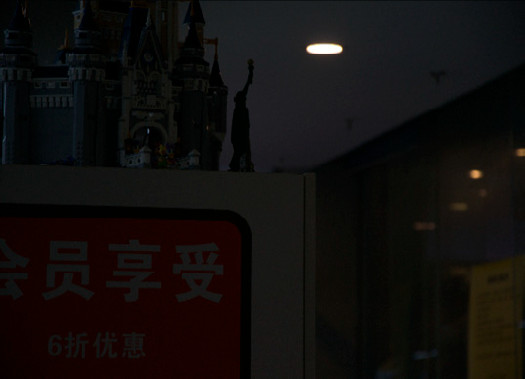
\includegraphics[width=\linewidth]{picture/LLIE/VE-LOL-L/input}
			\captionsetup{font=scriptsize}
			\caption*{input \\ \quad }
			\label{fig: input}
		\end{subfigure}
		\begin{subfigure}{0.17\columnwidth}
			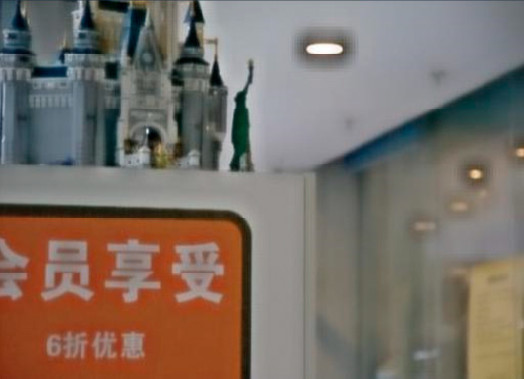
\includegraphics[width=\linewidth]{picture/LLIE/VE-LOL-L/LLNet}
			\captionsetup{font=scriptsize}
			\caption*{LLNet \\ (2017)}
			\label{fig: LLNet_VE_LOL}	
		\end{subfigure}
		\begin{subfigure}{0.17\columnwidth}
			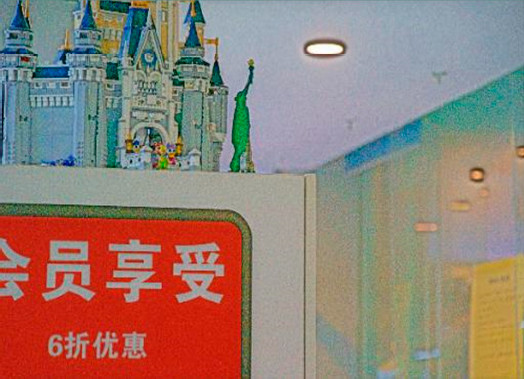
\includegraphics[width=\linewidth]{picture/LLIE/VE-LOL-L/RetinexNet}
			\captionsetup{font=scriptsize}
			\caption*{RetinexNet \\ (2018)}
			\label{fig: RetinexNet_VE_LOL}	
		\end{subfigure}
		\begin{subfigure}{0.17\columnwidth}
			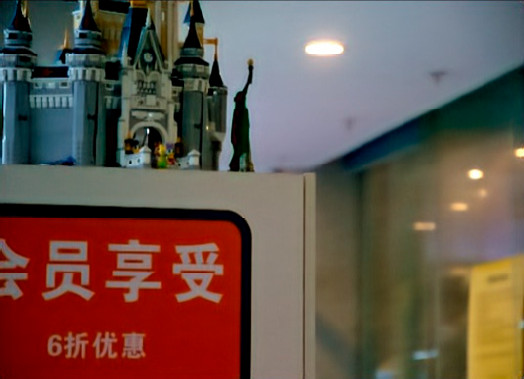
\includegraphics[width=\linewidth]{picture/LLIE/VE-LOL-L/MBLLEN}
			\captionsetup{font=scriptsize}
			\caption*{MBLLEN \\ (2018)}
			\label{fig: MBLLEN_LOL}	
		\end{subfigure}
		\begin{subfigure}{0.17\columnwidth}
			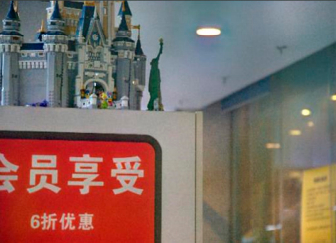
\includegraphics[width=\linewidth]{picture/LLIE/VE-LOL-L/EnlightenGAN}
			\captionsetup{font=scriptsize}
			\caption*{EnlightenGAN \\ (2019)}
			\label{fig: EnlightenGAN_VE_LOL}	
		\end{subfigure}
		\begin{subfigure}{0.17\columnwidth}
			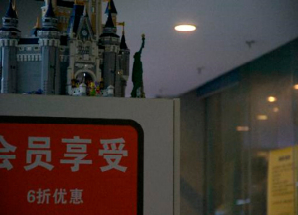
\includegraphics[width=\linewidth]{picture/LLIE/VE-LOL-L/RRDNet}
			\captionsetup{font=scriptsize}
			\caption*{RRDNet \\ (2020)}
			\label{fig: RRDNet_VE_LOL}	
		\end{subfigure}
		\begin{subfigure}{0.17\columnwidth}
			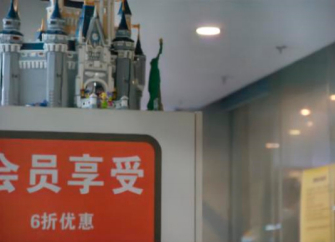
\includegraphics[width=\linewidth]{picture/LLIE/VE-LOL-L/DRBN}
			\captionsetup{font=scriptsize}
			\caption*{DRBN \\ (2020)}
			\label{fig: DRBN_VE_LOL}	
		\end{subfigure}
		\begin{subfigure}{0.17\columnwidth}
			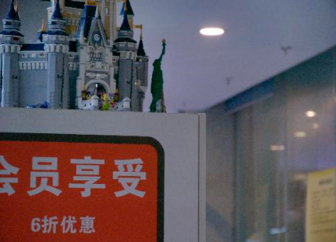
\includegraphics[width=\linewidth]{picture/LLIE/VE-LOL-L/Zero-DCE++}
			\captionsetup{font=scriptsize}
			\caption*{Zero-DCE++ \\ (2021)}
			\label{fig: Zero-DCE++}	
		\end{subfigure}
		\begin{subfigure}{0.17\columnwidth}
			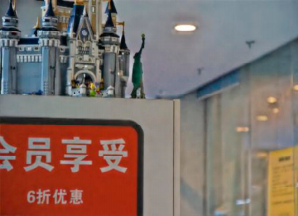
\includegraphics[width=\linewidth]{picture/LLIE/VE-LOL-L/KinD++}
			\captionsetup{font=scriptsize}
			\caption*{KinD++ \\ (2021)}
			\label{fig: KinD++}	
		\end{subfigure}
		\begin{subfigure}{0.17\columnwidth}
			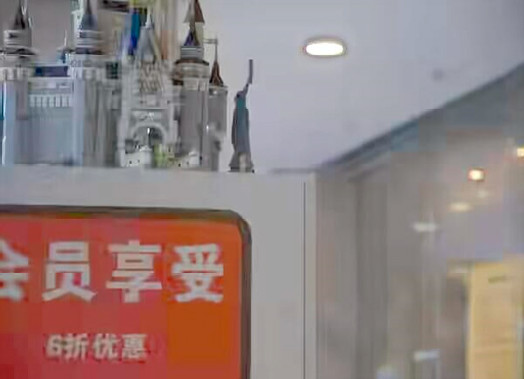
\includegraphics[width=\linewidth]{picture/LLIE/VE-LOL-L/URetinexNet}
			\captionsetup{font=scriptsize}
			\caption*{URetinexNet \\ (2022)}
			\label{fig: URetinexNet}	
		\end{subfigure}
		\caption{
			\label{fig: VE-LOL-L Visual} 
			不同算法对从 VE-LOL-L 数据集采样的低照度图像的可视化结果。 
		}
	\end{figure}
	
	近年来,基于深度学习的低光图像增强(LLIE)技术取得了显著成就,它使用神经网络来学习从弱光图像到自然光图像的映射。与传统方法相比,基于深度学习的解决方案在准确性、鲁棒性和处理速度方面表现更优,因此受到了广泛关注。特别是卷积神经网络(CNN)在多个计算机视觉任务中展现出卓越的性能。CNN通过利用注意力机制和\cite{yang2021locally, zhang2020attention}上下文信息,能够从原始图像中有效提取多尺度特征\cite{li2018multi, zamir2020learning}。在这些成果的推动下,基于CNN的低光图像增强方法得到了持续发展。例如,一种基于CNN的自适应低光图像增强框架\cite{li2020visual}显著提升了图像的对比度、颜色和细节信息。然而,现有的基于CNN的方法大多集中于图像亮度、纹理和颜色的恢复,对于局部光照不均匀、颜色信息和细节信息的丢失问题,仍存在过增强或增强不足的挑战。
	
	现有的方法可能无法在极暗或极亮的区域恢复图像边缘细节\cite{xu2023low},如图\ref{fig: SNR (CVPR 2022)}和图\ref{fig: SMG-LLIE}所示,暗区结构细节模糊。同时,当物体边缘不清晰时,像素级损失往往会模糊边缘,破坏图像细节。而加入边缘先验可以降低优化外观重构时的不适定程度。人类视觉系统对边缘高度敏感,保留结构信息对图像重建任务的性能至关重要。定义边缘可以通过学习区分黑暗区域的不同物体来指导增强过程,而不仅仅是识别低光区域。通过保留图像中的结构属性,这使得物体之间的可见性更好。
	
	\begin{figure}[htb]
		\centering
		\begin{subfigure}{0.45\columnwidth}
			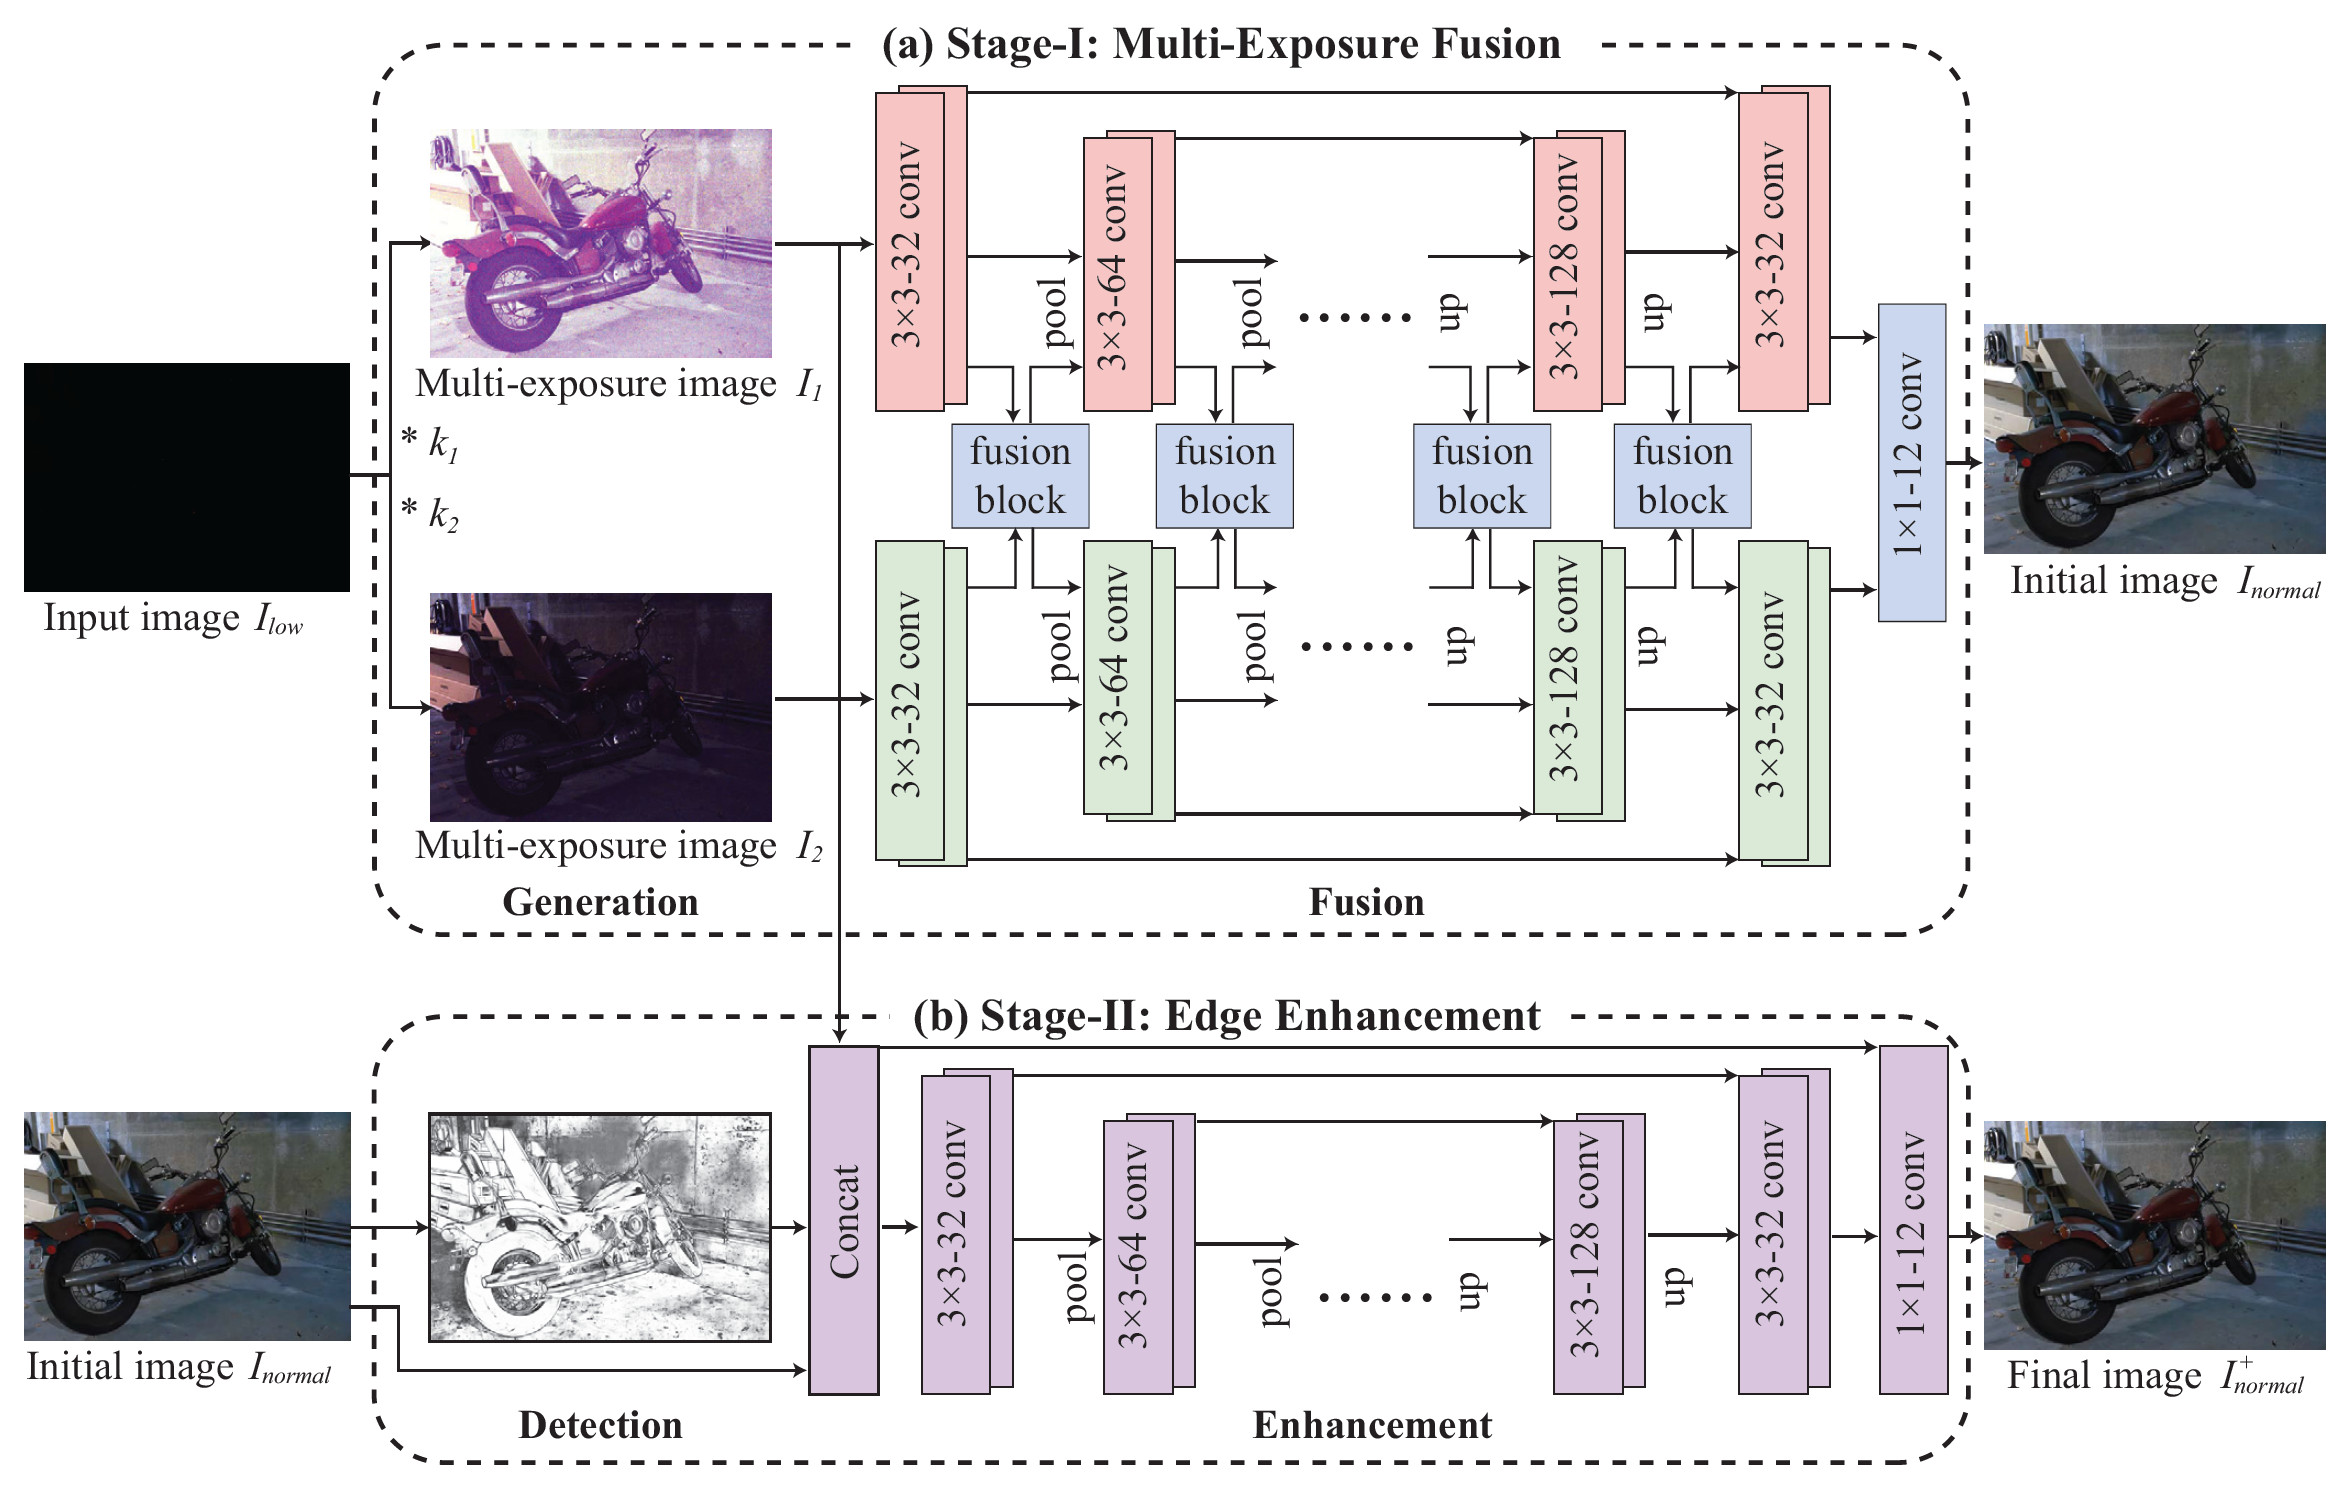
\includegraphics[width=\linewidth]{picture/LLIE/EEMEFN/EEMEFN framework}
			\captionsetup{font=scriptsize}
			\caption{\label{fig: EEMEFN}
				该 LLIE 结构源自\cite{zhu2020eemefn},如其 Multi-Exposure Fusion 部分采用多曝光融合结构,与由 Initial image 生成的边缘图进行 Concat, 后续通过一个 U-Net 网络进一步恢复图像。}
		\end{subfigure}
		\begin{subfigure}{0.45\columnwidth}
			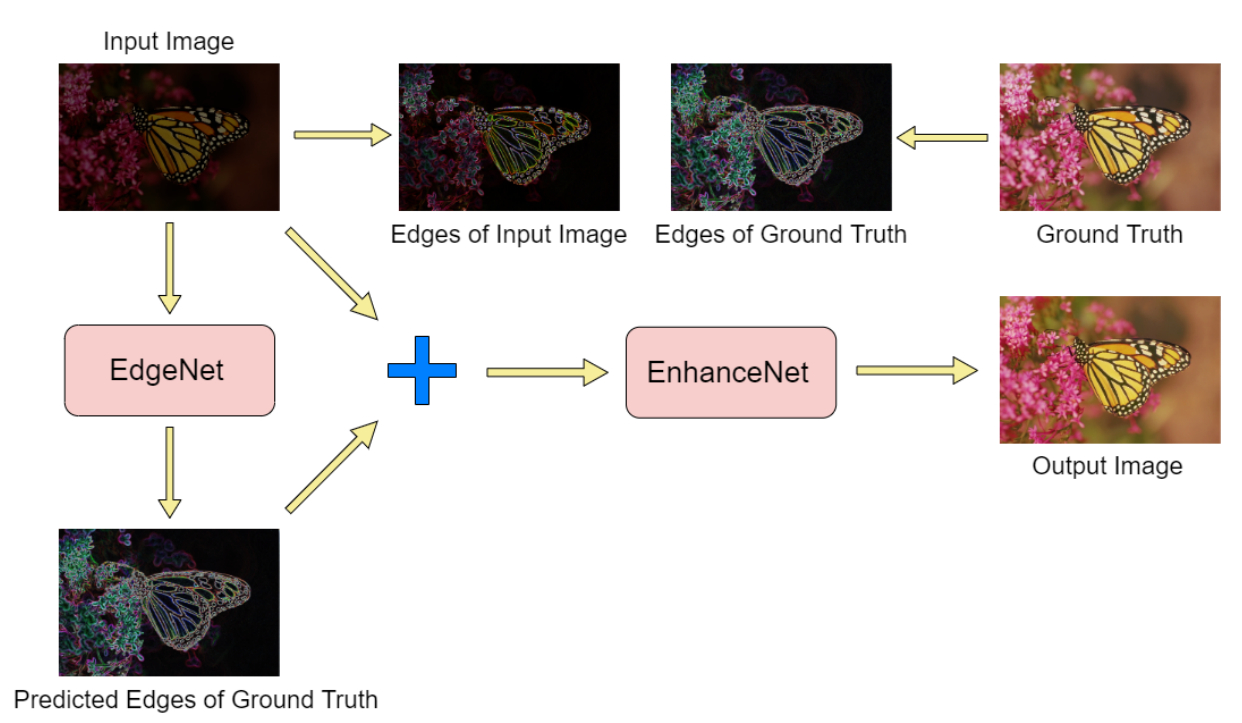
\includegraphics[width=\linewidth]{picture/LLIE/EdgeNet/Archtecture workflow}
			\captionsetup{font=scriptsize}
			\caption{\label{fig: EdgeNet} 
				该 LLIE 结构源自\cite{rana2021edge}使用 EdgeNet 首先从低光图像中过滤边缘,EnhanceNet 反复使用上采样和下采样块的组合,从局部到全局逐渐提取特征,并消除伪影和噪声。}
		\end{subfigure}
		\caption{
			\label{fig: Traditional Architecture}
			边缘图像指导弱光图像增强的传统架构。
		}
	\end{figure}
	
	\begin{figure}[htb]
		\centering 
		\begin{subfigure}{0.8\columnwidth}
			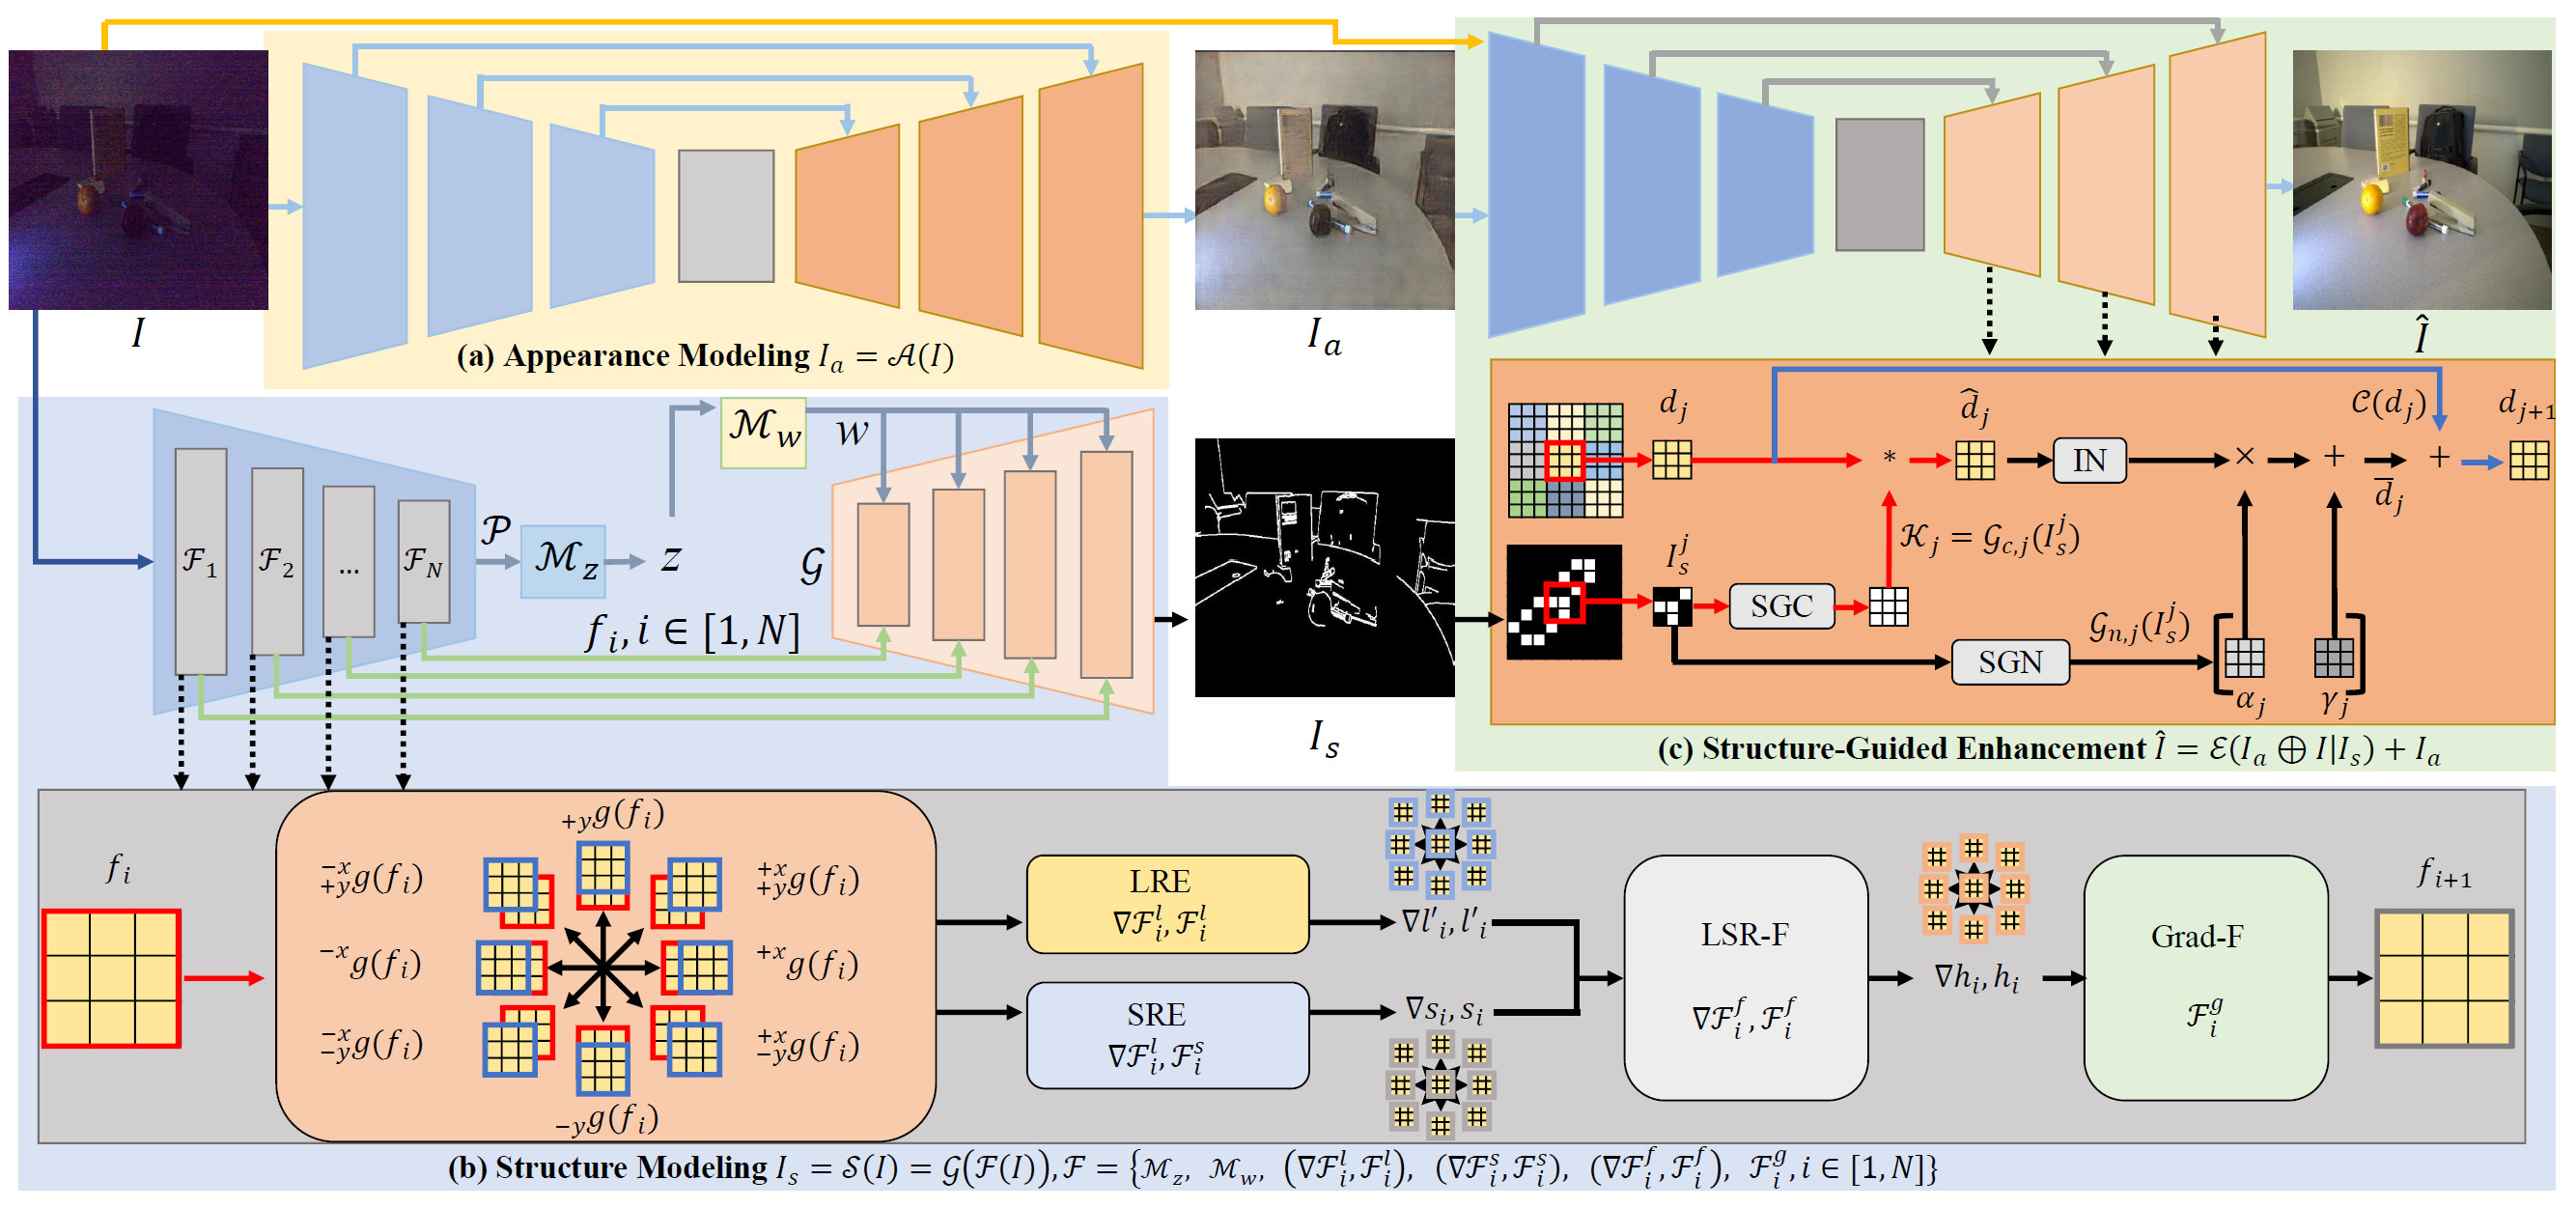
\includegraphics[width=\columnwidth]{picture/LLIE/Structure Modeling and Guidance/Overview}
			\captionsetup{font=scriptsize}
			\caption{该 LLIE 结构源自\cite{xu2023low},其提出一种基于 GAN Loss 的模型去对结构信息建模,通过获得的结构信息指导增强。}
			\label{fig: SMG-LLIE Architecture}
		\end{subfigure}
		\caption{
			\label{fig: SMG-LLIE Overview} 
			边缘图像指导弱光图像增强的最新架构(CVPR 2023)。
		}
	\end{figure}
	
	\begin{figure}[htb]
		\centering
		\begin{subfigure}{0.25\columnwidth}
			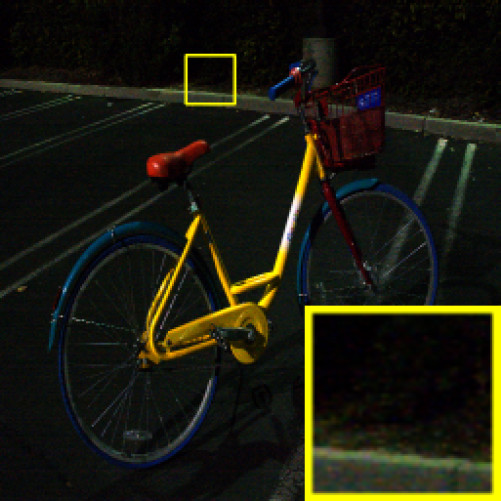
\includegraphics[width=\linewidth]{picture/LLIE/Structure Modeling and Guidance/Input}
			\captionsetup{font=scriptsize}
			\caption{Input}
			\label{fig: Input}
		\end{subfigure}
		\begin{subfigure}{0.25\columnwidth}
			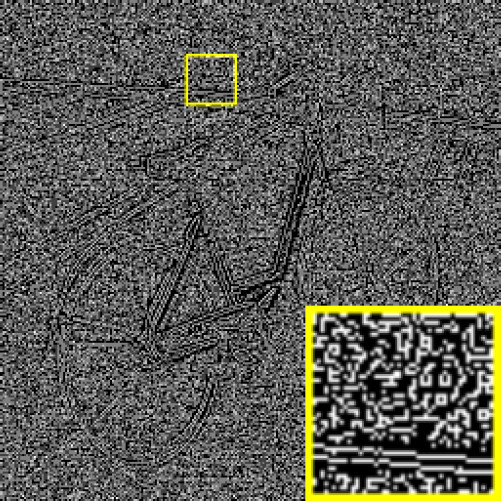
\includegraphics[width=\linewidth]{picture/LLIE/Structure Modeling and Guidance/Structure of (a)}
			\captionsetup{font=scriptsize}
			\caption{Structure of (a)}
			\label{fig: Structure of (a)}	
		\end{subfigure}
		\begin{subfigure}{0.25\columnwidth}
			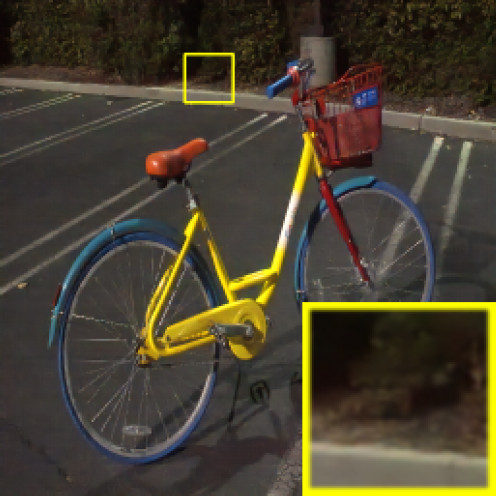
\includegraphics[width=\linewidth]{picture/LLIE/Structure Modeling and Guidance/SNR (CVPR 2022)}
			\captionsetup{font=scriptsize}
			\caption{SNR (CVPR 2022)}
			\label{fig: SNR (CVPR 2022)}	
		\end{subfigure}
		\begin{subfigure}{0.25\columnwidth}
			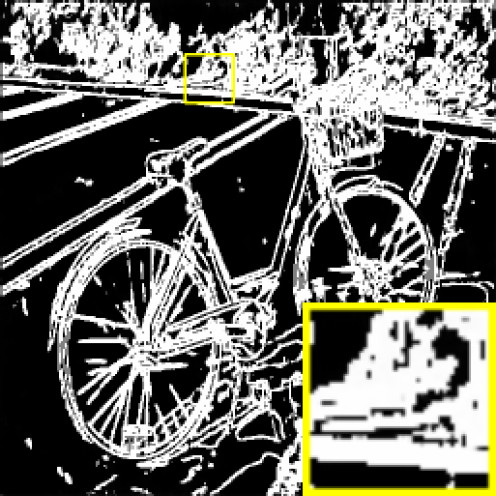
\includegraphics[width=\linewidth]{picture/LLIE/Structure Modeling and Guidance/Structure Modeling}
			\captionsetup{font=scriptsize}
			\caption{Structure Modeling}
			\label{fig: Structure Modeling}
		\end{subfigure}
		\begin{subfigure}{0.25\columnwidth}
			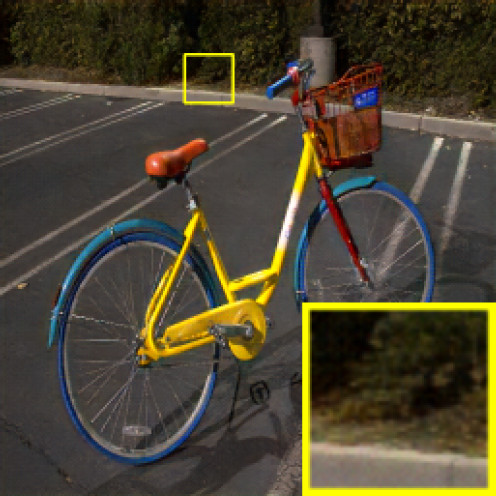
\includegraphics[width=\linewidth]{picture/LLIE/Structure Modeling and Guidance/Ours}
			\captionsetup{font=scriptsize}
			\caption{SMG-LLIE}
			\label{fig: SMG-LLIE}
		\end{subfigure}
		\begin{subfigure}{0.25\columnwidth}
			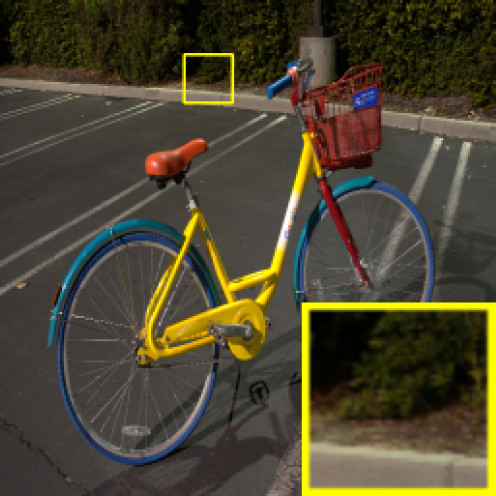
\includegraphics[width=\linewidth]{picture/LLIE/Structure Modeling and Guidance/Ground Truth}
			\captionsetup{font=scriptsize}
			\caption{Ground Truth}
			\label{fig: Ground Truth}
		\end{subfigure}
		\caption{
			\label{fig: Structural Information}
			SID-sRGB\cite{chen2018learning}中一张弱光图片, 通过SOTA方法 (c) 和\cite{xu2023low}提出的方法 (e)增强。作者的方法可以从输入的图像中合成结构图(d),使细节更清晰,对比度更清晰,颜色更鲜艳。虽然(c)的 PSNR 为 28.17,但其 SSIM 低为 0.75。作者的方法在dB和SSIM\cite{wang2004image}的得分都很高,分别为28.60 dB 和 0.80。
		}
	\end{figure}
	
	基于这个问题,即\textbf{如何更好的使用边缘图来“指导”弱光图像的恢复?}我们对此进行了相关文献调研。其中,一类方法(如图\ref{fig: Traditional Architecture}所示,我们称之为传统架构)是采用边缘检测思想来引导弱光图像增强,其策略是将边缘图与\textbf{一张从弱光中初步恢复的图像}(后面统一称作初步恢复图像)进行串联,然后通过一个增强网络来实现最终的图像增强\cite{zhu2020eemefn, rana2021edge}。但是我们通过观察这类模型的架构发现其具有以下三个特点:
	
	\begin{itemize}
		\item [(1)] 其恢复结果的质量往往会受到最后的增强网络设计和初步恢复图像所包含特征与真实图像特征之间的相似度的影响。
		
		\item [(2)] 边缘图的准确性会极大影响最终的恢复结果,直接从弱光图像中获取边缘图具有一定的挑战性。
		
		\item [(3)] 边缘图与初步恢复图像之间多采用串联方式输入卷积以获得最终增强结果。
	\end{itemize}
	
	传统架构存在一定的局限性,虽然采用了边缘结构信息增强弱光图像,但是无法很好的利用边缘信息语义指导恢复弱光图像,需要在现有的直接串联方法的基础上进行改进。此外,从低光照中的图片很难提取到好的结构信息,如何设计更好的边缘网络从弱光图像中提取出接近 GT 边缘图的结果是我们需要考虑的问题。
	
	作者\cite{xu2023low}提出了一种基于结构先验的图像增强方式,以更好的从弱光图像中提取到更有效的边缘信息并用于指导图像增强。从图\ref{fig: Structural Information}中可以看到边缘图和LBP图\cite{pietikainen2010local}所反映结构信息具有明显的区别,边缘信息能反映更多的细节信息。我们不难发现,相较于LBP,图像边缘图仅保留了很少的数据量,其剔除了不相关的信息,保留了图像重要的结构属性。人类视觉系统对边缘高度敏感,保留结构信息对图像重建任务的性能至关重要。定义边缘可以通过学习区分黑暗区域的不同物体来指导增强过程,而不仅仅是识别低光区域。通过保留图像中的结构属性,这使得物体之间的可见性更好。
	
	此外,获取边缘图的方法也各不相同,在 LLIE 任务中,常见方法采用边缘检测网络来生成边缘图,然后使用 Canny 或 Sobel 算子\cite{maini2009study}从 GT 中获取边缘图用做对照组。目前在 LLIE 领域中获取边缘图分化成了两个不同的方向,一种是通过初步恢复图像获取边缘图(见图\ref{fig: EEMEFN}),另一种是直接通过弱光图像以获取边缘图(见图\ref{fig: EdgeNet}和图\ref{fig: SMG-LLIE Architecture})。LLIE 任务中边缘检测的主要有下列方法:
	
	\begin{itemize}
		\item [(1)] 手工设计各种滤波器来生成边缘图。
		
		\item [(2)] 根据人类设计的特征使用数据驱动模型来预测边缘(随机决策森林来学习边缘板块)。
		
		\item [(3)] 深度学习方法从原始数据中学习复杂的特征表示端到端边缘检测模型(RCF边缘检测模型\cite{liu2017richer})。
	\end{itemize}
	
	综上所述,本研究旨在实现以下明确的研究目标\footnote{在对Xu等人\cite{xu2023low}的模型(参见图\ref{fig: SMG-LLIE Architecture})进行深入分析后,本研究旨在通过采用与原作者不同的方法论来实现若干具体目标,并力求在关键评价指标上超越原模型的性能。具体而言,本研究的核心目标包括:首先,在目标(1)和目标(2)的框架内,探索与Xu等人不同的优化策略;其次,这些优化策略应致力于提升模型的整体性能,目的在于在关键评价指标上实现超越原作者的成果。通过这种方法,本研究不仅旨在增强现有模型的能力,同时也寻求对该领域的理论和实践知识做出贡献。}:
	
	\begin{itemize}
		\item [(1)] \textbf{边缘网络的开发:} 设计并构建一个创新的边缘网络,其核心功能是从低光照图像中直接提取边缘结构图。该网络生成的结构图应与地面真实(GT)生成的边缘结构图具有高度的相似性,从而确保准确性和可靠性。
		
		\item [(2)] \textbf{初步恢复图像的生成模型:} 开发一个用于生成初步恢复图像的低光照图像增强模型。该模型应专注于从弱光条件下的图像中恢复清晰度和细节,以提高整体图像质量。
		
		\item [(2)] \textbf{边缘语义信息的增强网络模型:} 在现有的直接串联方法基础上,进行创新性改进,构建一种更有效利用边缘语义信息的增强网络模型。目的在于通过这种改进,进一步提升图像增强过程中边缘结构的利用效率和效果。
	\end{itemize}
	
	通过实现这些目标,本研究期望对低照度图像处理领域的理论与实践作出贡献,特别是在图像边缘结构的提取和利用方面。
	
	\part*{研究内容}
	
	\section{采用的方法}
	
	在初步恢复图的生成方面,我们受到了 Conformer 结构\cite{peng2021conformer}的启发,该结构巧妙地结合了卷积神经网络(CNN)在捕获短距离特征\cite{jain1991unsupervised, lowe2004distinctive, ojala2002multiresolution}方面的优势与Transformer自注意力模块在捕获长距离特征\cite{lisin2005combining}依赖关系方面的能力。然而,Transformer的自注意力模块在捕获远距离特征的同时,可能会忽视局部特征的细节。为了克服这一局限性,Conformer结构融合了卷积运算和自注意力机制,以增强表示学习的能力。在此基础上,我们提出一种新颖的并行深度学习架构,专门针对低光照条件下的图像增强问题。该模型融合了经典的 U 型网络和 Transformer 深度学习方法,旨在提升弱光图像增强任务中恢复图像的可视性和质量,同时保留关键的细节和纹理信息。
	\section{数据集}
	
	\section{文献调研与支撑}
	
	\part*{具体工作内容}
	
	\section{已完成工作}
	
	\section{下一步工作}
	
	在计算机视觉领域,研究人员使用了不同类型的注意力机制,目的是使模型聚焦于图像本身。这大致分为两种类型:一种是基于通道的注意力机制,即 Squeeze-and-Excite。另一个是基于空间的注意力机制\cite{woo2018cbam}。然而,研究发现这些类型有三个局限性:
	
	\begin{itemize}
		\item[(1)] 
		卷积捕捉远距离特征的能力较差;
		
		\item[(2)]
		注意力机制关注所有输入;当分辨率较大时,计算成本增加;
		
		\item[(3)]
		不同时关注通道和空间维度关注信息。这就造成了信息的浪费和注意力的减弱。
	\end{itemize}	
	
	针对第一个限制 \cite{ramachandran2019stand} 将所有卷积替换为独立的自注意层和空间意识的独立自注意层,替换后的模型为纯注意模型。纯注意模型增强了网络对远距离特征连接的建模能力。在 ImageNet分类任务和 COCO 对象检测任务中,该模型优于使用卷积的基线模型。对于第三个限制,Woo 等人\cite{woo2018cbam}提出了一种卷积块注意模型 CBAM,这是一种轻量级的通用注意模型。该模型从通道维度和空间维度两方面关注重要信息。由于 CBAM 从多个维度提取重要信息,该模型被广泛应用于目标检测、目标分类等任务。实验表明,CBAM 模块可以显著提高网络的表达能力。同时,CBAM 可以搭配 SCConv\cite{li2023scconv}结构,SCConv 是一种名为可以即插即用的卷积模块,目的是减少卷积神经网络中特征之间的空间和通道冗余,从而压缩 CNN 模型并提高其性能。
	
	\paragraph{U-Net for LLIE}
	
	U-Net 网络由卷积层、下采样、上采样和跳过连接操作组成,其编码器和解码器具有对称结构。长期以来,U-Net 网络及其改进结构由于其强大的特征学习和特征重构能力,在图像语义分割领域取得了巨大的成功。U-Net 网络在弱光图像增强方面显示出出色的效果。Chen 等\cite{chen2018learning}创新性地提出了一种基于 U-Net 框架的弱光图像增强网络。该网络的核心架构是多尺度上下文聚合网络 (CAN) 和 U-Net 网络。之后的工作\cite{chen2018learning, zamir2021learning}也将 U-Net 架构应用到自己的网络中,其网络包含两个子网。即图像约简子网和感知损失子网,其中图像约简子网具有与\cite{chen2018learning}相同的 U-Net 架构。虽然\cite{chen2018learning, zamir2021learning}在使用U-Net架构增强图像方面取得了一定的效果,但\cite{meng2020gia}认为\cite{chen2018learning, zamir2021learning}网络忽略了全局信息,导致增强图像中的颜色不自然和物体伪影问题。为了改善以往网络的缺陷,利用 U-Net 架构,\cite{meng2020gia}在U-Net的编码器和解码器之间增加了全局信息感知模块(global information awareness module, GIA), GIA 可以将全局信息整合到整个网络中,改善增强图像中的颜色不一致和伪影。经过对\cite{chen2018learning, meng2020gia, zamir2021learning}的仔细研究,基于 U-Net 网络的弱光图像增强方法取得了很好的效果。然而,该网络仍然存在两个局限性:
	
	\begin{itemize}
		\item[(a)] 
		跳过连接只融合相同尺度的特征,导致编码器和解码器之间存在较大的语义差距;
		
		\item[(2)]
		全局上下文信息的连接相对稀缺。
	\end{itemize}	
	
	这两个限制容易导致增强图像的细节丢失、对比度差和颜色信息不准确。Zhou等\cite{zhou2018unet++,zhou2019unet++}改进了 U-Net 架构生成 U-Net++,在 U-Net++ 中将跳跃连接重新设计为一系列嵌套的密集跳跃连接,实现了多个特征的融合,加强了不同层次的特征信息接触。
	
	\paragraph{CNN for LLIE}
	
	CNN 在许多计算机视觉任务中表现出了令人印象深刻的结果。CNN 利用注意力机制\cite{yang2021locally, zhang2020attention}和上下文信息,从原始图像中生成注意感知并提取多尺度特征\cite{li2018multi,zamir2020learning}。基于 CNN 的低光图像增强方法不断发展。例如,基于 CNN 的自适应弱光图像增强框架\cite{li2020visual}极大地增强了图像对比度、颜色和细节信息。然而,现有的基于 CNN 的方法大多侧重于图像亮度、纹理和颜色的恢复\cite{xu2020learning}。由于局部光照不均匀,颜色信息和细节信息丢失严重,容易出现过增强或增强不足的问题。
	
	\section{方向}
	
	根据目前的文献研究,在 LLIE 任务中,一种方法是采用边缘检测思想来引导弱光图像增强\footnote{为什么要采用图像的边缘图片来指导弱光图像恢复?
		首先,图像边缘图仅需要很少的数据量,其剔除了不相关的信息,保留了图像重要的结构属性。其次,低光图像通常具有很高的对比度,现有的方法可能无法在极暗或极亮的区域恢复图像边缘细节。同时,当物体边缘不清晰时,像素级损失往往会模糊边缘,破坏图像细节。而加入边缘先验可以降低优化外观重构时的不适定程度。最后,人类视觉系统对边缘高度敏感,保留结构信息对图像重建任务的性能至关重要。定义边缘可以通过学习区分黑暗区域的不同物体来指导增强过程,而不仅仅是识别低光区域。通过保留图像中的结构属性,这使得物体之间的可见性更好。},其策略是将边缘图与\textbf{初步恢复的图像}进行串联,然后通过单一的增强网络来实现最终的图像恢复。恢复结果的质量往往会受到最后的增强网络设计和初步恢复图像所包含特征与真实图像特征之间的相似度的影响。
	
	根据目前的文献调研,当前的此类方法的特点只集中在通过边缘图指导图像恢复,且恢复出来的图像还是有明显噪点。
	
	\subsection{方向一}
	
	\textbf{图像初步恢复的方法}目前主要包括以下几种:
	
	\begin{itemize}
		\item[(1)] 
		利用多曝光技术\footnote{多曝光技术已被实验证明可以有效的解决 LLIE 任务中普遍存在的色彩失真问题。}获得具有不同曝光度的图像,然后结合恢复网络进行初步恢复\footnote{常见的架构如基于 GAN 的多曝光图像融合架构,基于端到端深度学习框架下多曝光图像融合算法,基于稀疏表示和可平移复方向金字塔变换的多曝光融合框架。};
		
		\item[(2)]
		结合 CNN 和 Transformer 架构的方法,可以是类似于 Uformer \cite{wang2022uformer}的串行架构,亦或者是类似于 Conformer 的并行架构。我们提出的 CNN 和 Transformer 并行架构(见Fig. \ref{fig: The proposed architecture})。
		
		\item[(3)]
		直接通过神经网络进行弱恢复。
		
	\end{itemize}	
	
	但由于噪声和伪影的存在,以及色彩与真实图像之间的差异,直接采用神经网络恢复结果通常并不理想。
	
	\begin{figure}[htbp]
		% read manual to see what [ht] means and for other possible options
		\centering 
		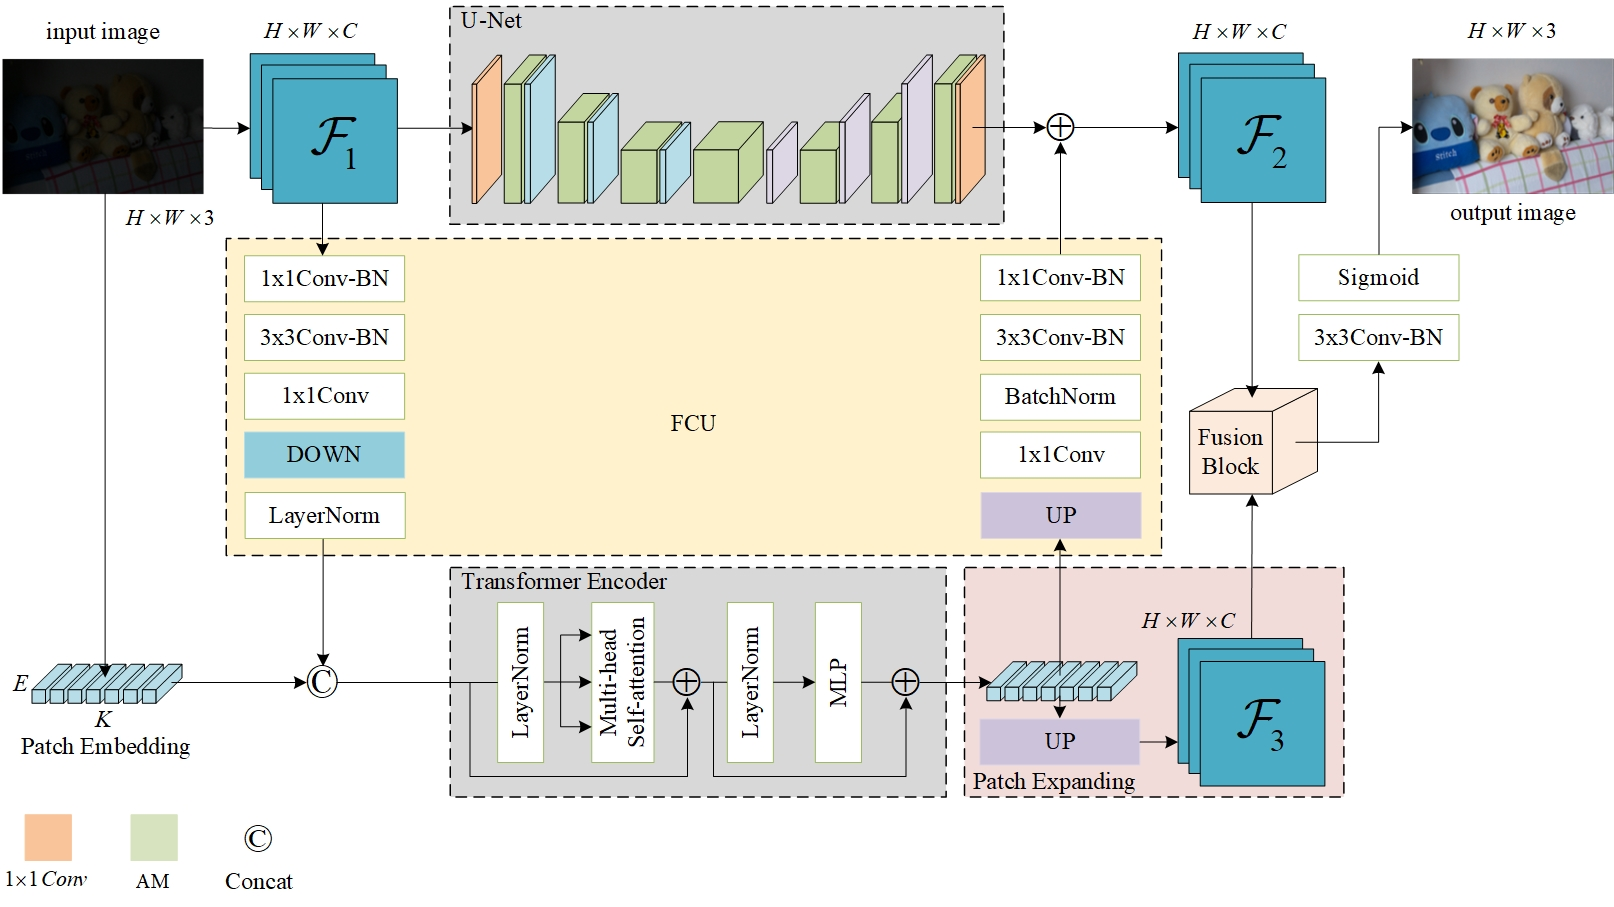
\includegraphics[width=\columnwidth]{picture/LLIE/My Architecture/The proposed initial architecture}
		%\captionsetup{font=scriptsize}
		\caption{
			\label{fig: The proposed architecture} 
			Low-Lighting 图像恢复网络。结构受 Conformer\cite{peng2021conformer} (见 Fig. \ref{fig: Conformer architecture})启发,将原来结构中 CNN 分支的 ResNet 结构修改为 U-Net 结构。其采用一个 U-Net 和 ViT 的并行架构,通过 U-Net 结构得到一个弱恢复的弱特征图 $\mathcal{F}_2$,通过 ViT 融合的特征可以初步增强弱特征图 $\mathcal{F}_2$,ViT 的输出经过 Patch Expanding 的特征图 $\mathcal{F}_3$ 经过与 U-Net 输出的特征图 $\mathcal{F}_2$ 融合之后得到一个初步恢复的图片 output image,用以后续参与图片的进一步恢复。
		}
	\end{figure}
	
	\textcolor{blue}{要求复现 Uformer\cite{wang2022uformer} 代码(见 Fig. \ref{fig: Uformer}),以及基于 Uformer 架构的改进方法\cite{li2023effective}。复现论文\cite{li2023effective}中提出的一种改进的基于 U-Net 网络的弱光图像增强方法(见 Fig. \ref{fig: MCLNet}),作者提出的 CEM 模块本质上基于 Uformer 思想。}。	
	\textcolor{red}{建议拟题《一种基于xx方法的弱光图像增强方法》}
	
	\begin{figure}[htbp]
		% read manual to see what [ht] means and for other possible options
		\centering 
		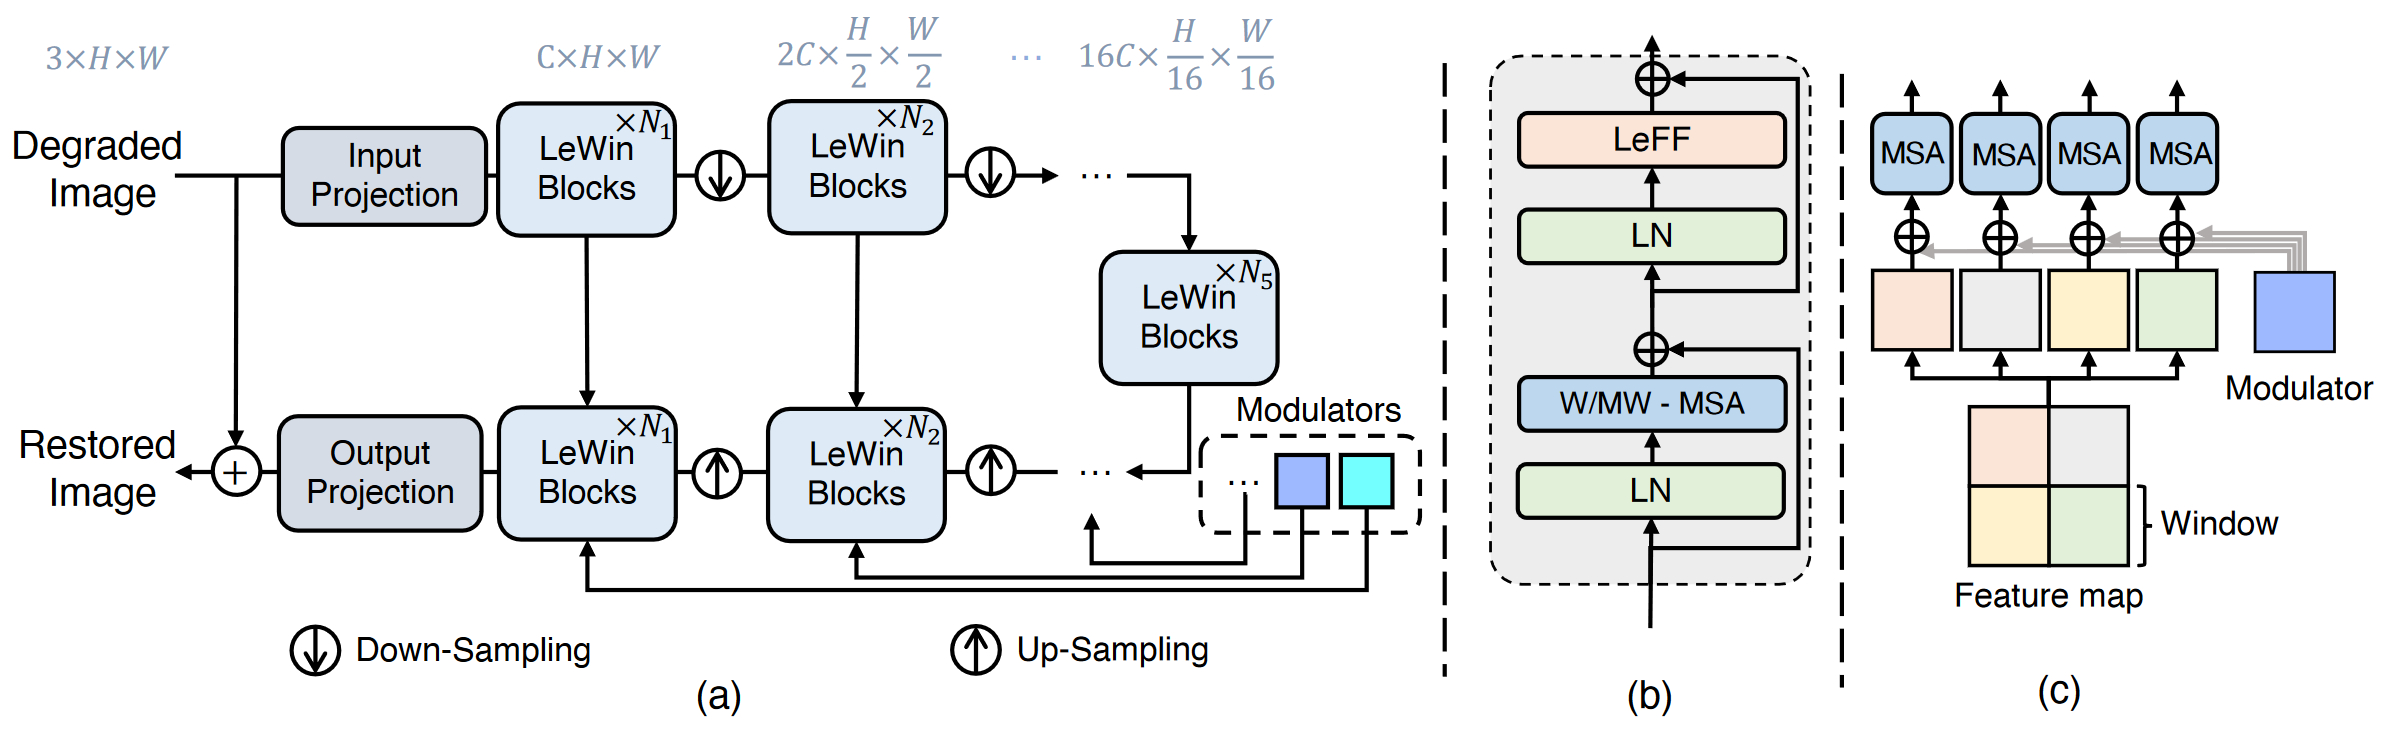
\includegraphics[width=\columnwidth]{picture/LLIE/Uformer/Uformer}
		%\captionsetup{font=scriptsize}
		\caption{
			\label{fig: Uformer} 
			Uformer 的结构。
		}
	\end{figure}
	
	\begin{figure}[htbp]
		% read manual to see what [ht] means and for other possible options
		\centering 
		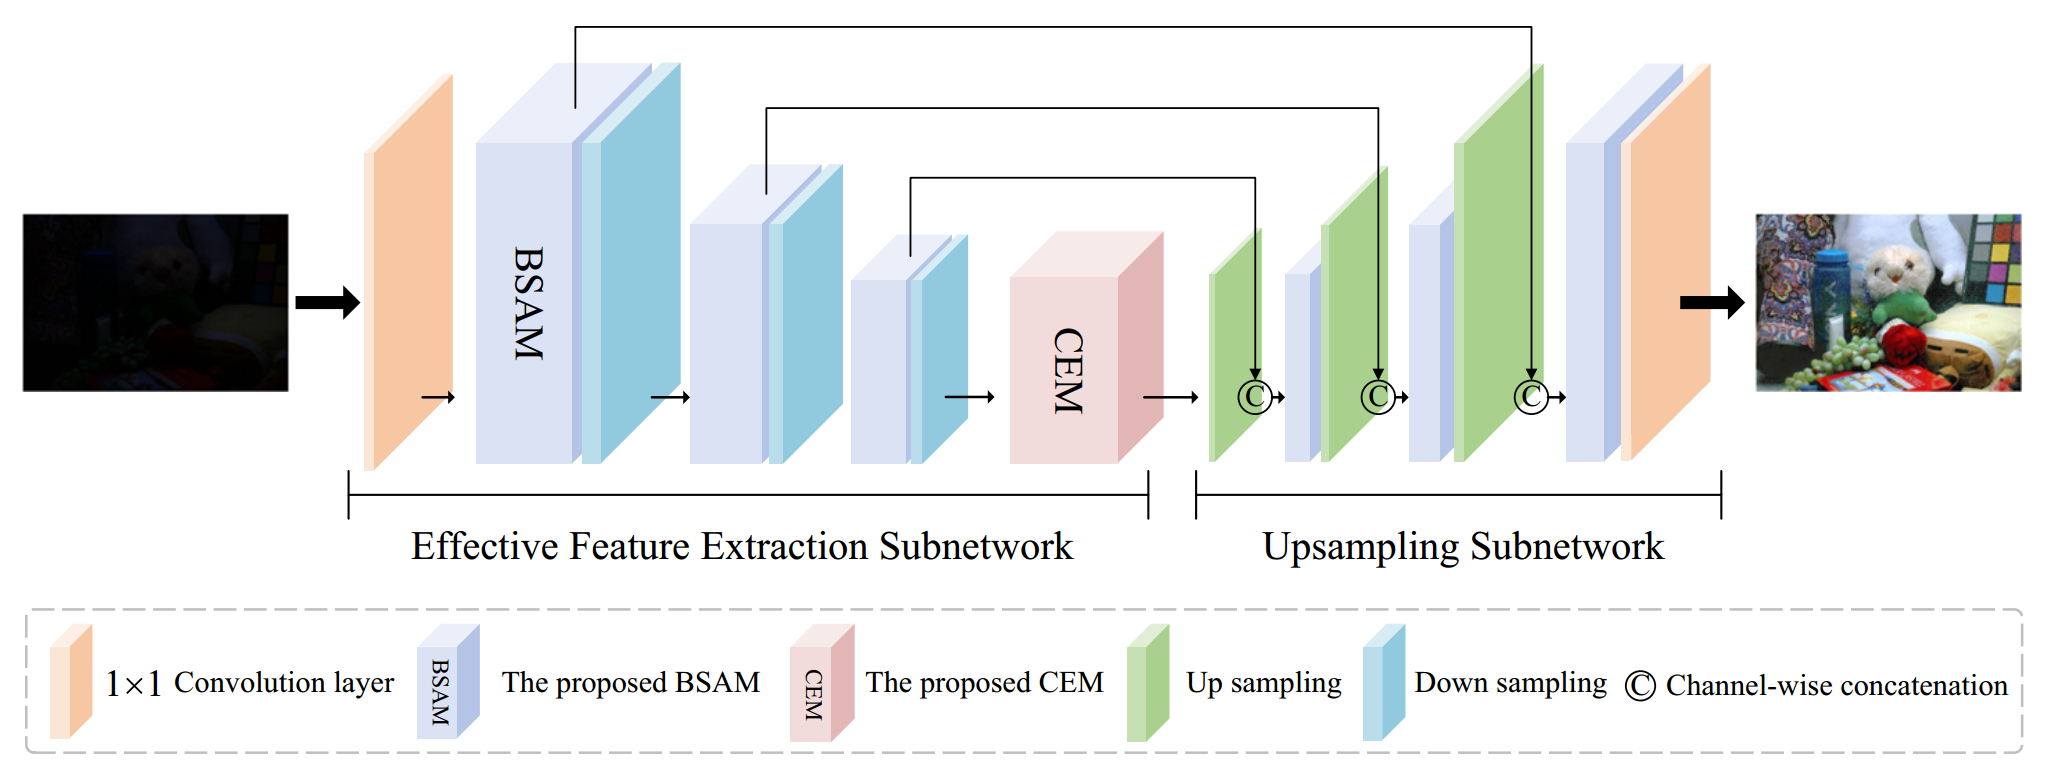
\includegraphics[width=\columnwidth]{picture/LLIE/MCLNet/Overview}
		%\captionsetup{font=scriptsize}
		\caption{
			\label{fig: MCLNet} 
			MCLNet 的结构
		}
	\end{figure}
	
	\subsection{方向二}
	
	此外,\textbf{获取边缘图的方法}也各不相同,在 LLIE 任务中,常见方法采用\textbf{边缘检测网络}来生成边缘图。Canny 和 Sobel 算子通常被用作对比实验,也有一些研究采用辅助边缘网络以提高边缘图生成的准确性。这些方法在弱光图像恢复研究中都具有一定的学术和实际应用价值。目前在 LLIE 领域中获取边缘图分化成了两个不同的方向,一种是采用初步恢复图像获取边缘图(如Fig. \ref{fig: EEMEFN}),另一种是直接采用弱光图像获取边缘图。
	
	\begin{figure}[htbp]
		% read manual to see what [ht] means and for other possible options
		\centering 
		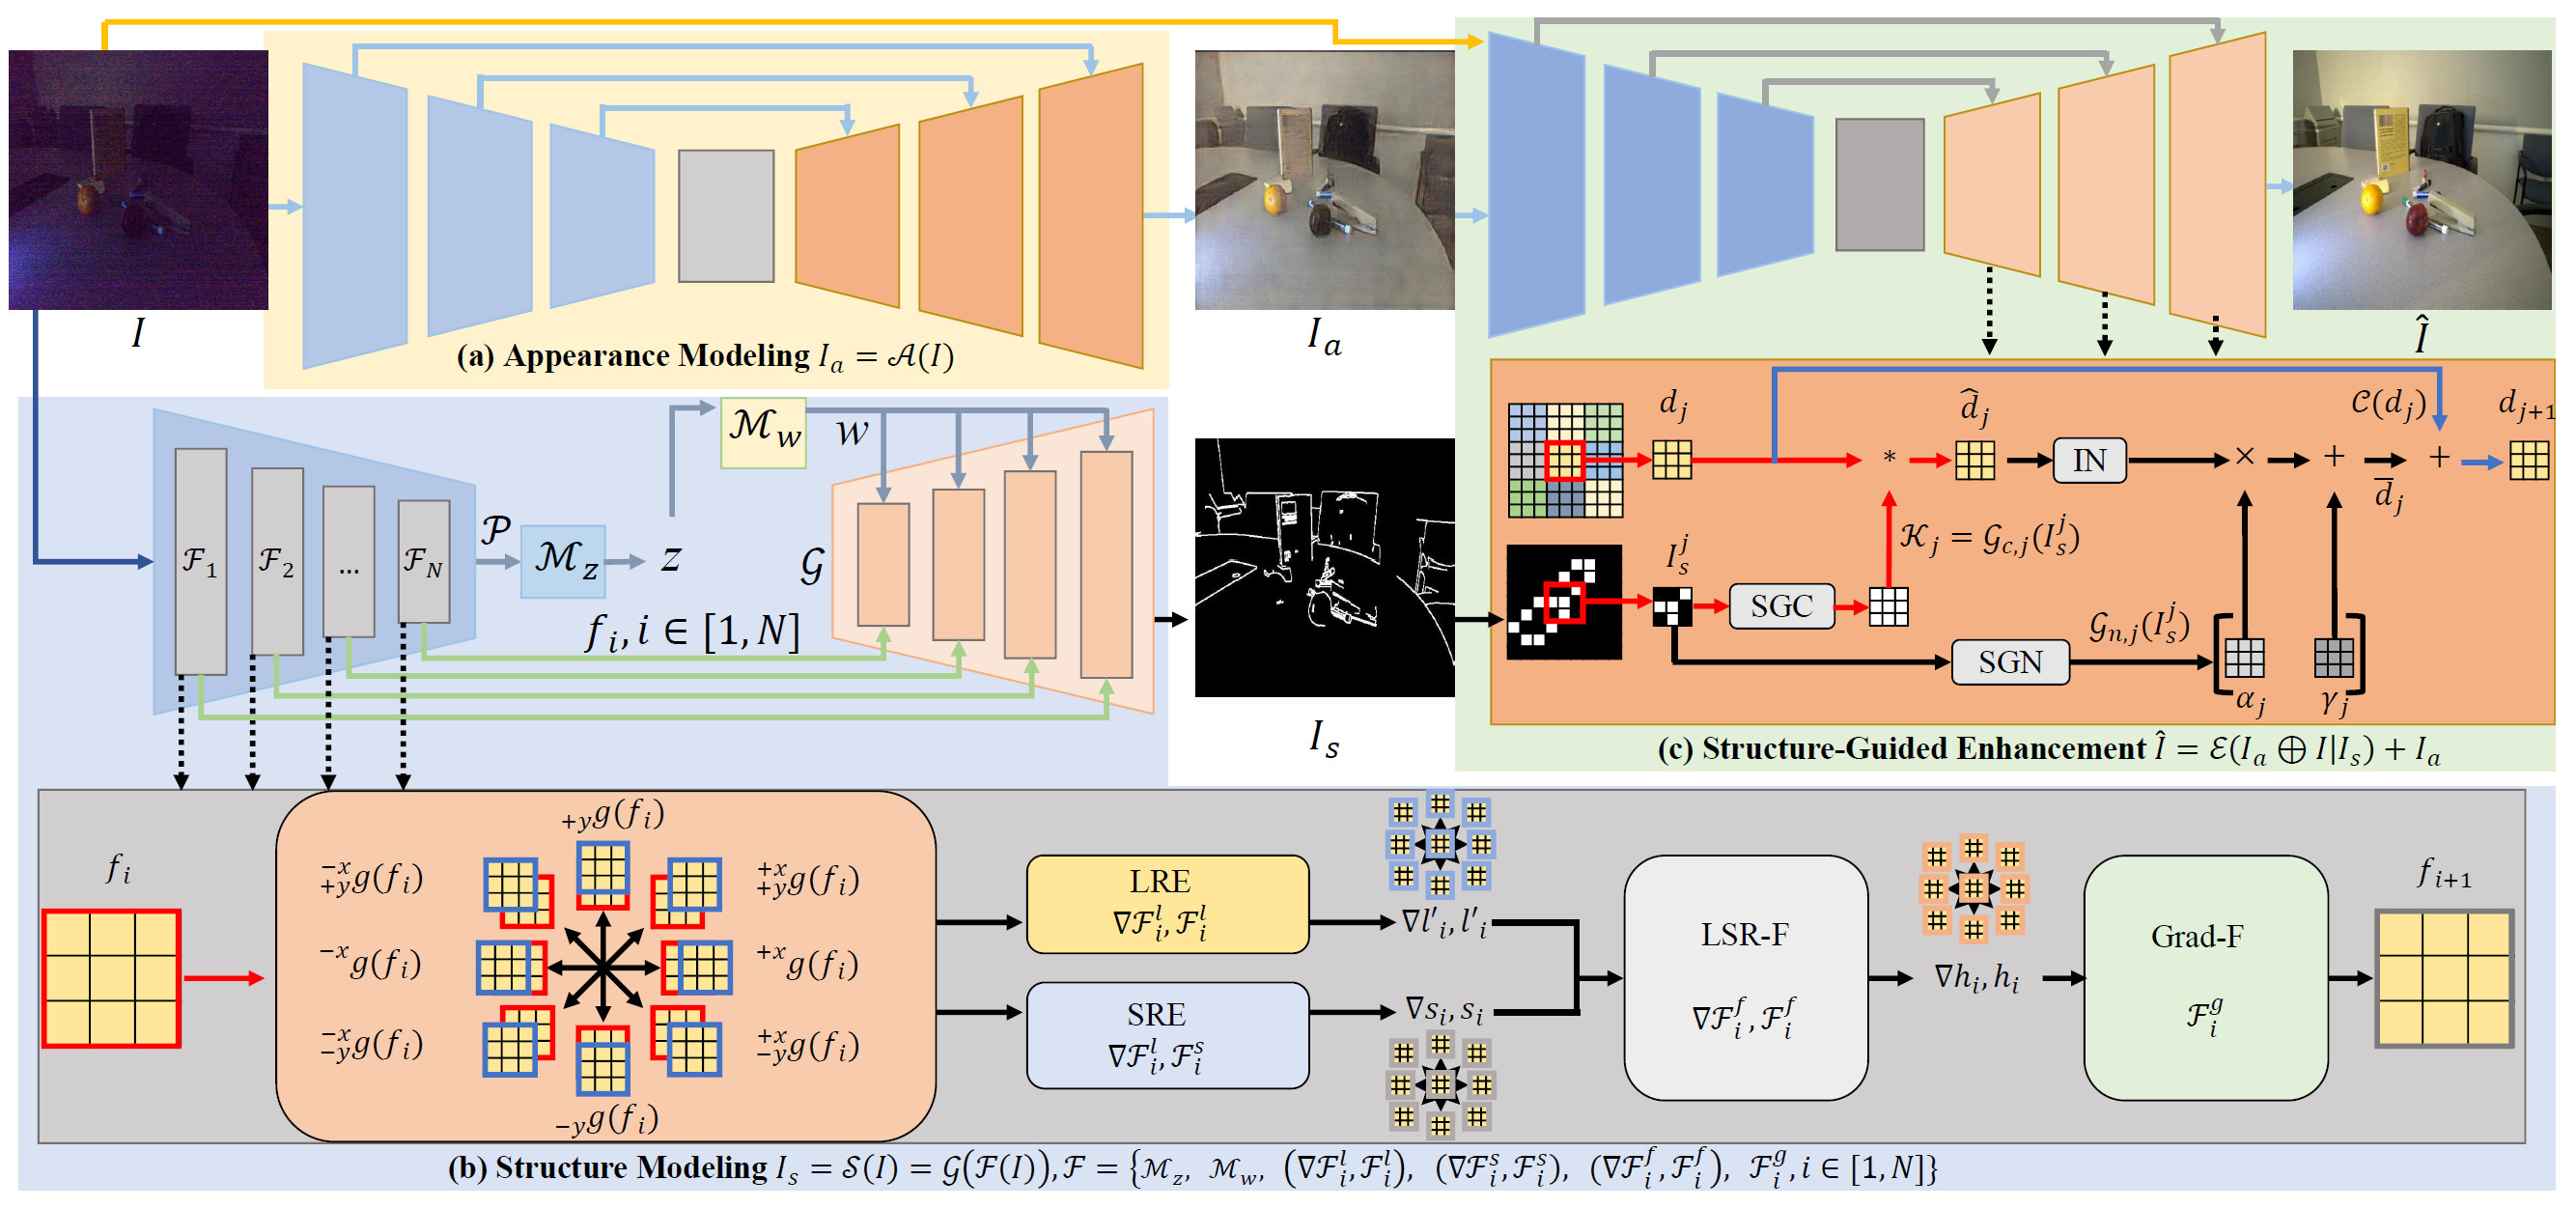
\includegraphics[width=\columnwidth]{picture/LLIE/Structure Modeling and Guidance/Overview}
		%\captionsetup{font=scriptsize}
		\caption{
			\label{fig: Overview} 
			该结构的边缘图直接从 $I$ 中通过 StyleGAN 得到边缘图 $I_s$, 而非从 $I_{\alpha}$ 中通过边缘网络获取边缘图。
		}
	\end{figure}
	
	图像处理任务中边缘检测的各种方法:
	
	\begin{itemize}
		\item[(1)] 
		手工设计各种滤波器来生成边缘图。
		
		\item[(2)]
		根据人类设计的特征使用数据驱动模型来预测边缘(随机决策森林来学习边缘斑块)
		
		\item[(3)]
		深度学习方法从原始数据中学习复杂的特征表示端到端边缘检测模型。
	\end{itemize}	
	
	\textcolor{blue}{要求复现论文\cite{xu2023low}代码。论文作者使用 StyleGAN 结构构建一种边缘网络,可以从弱光图像中获取边缘图。复现论文\cite{zhu2020eemefn}代码,其提出了一个从已经初步恢复的图像(非弱光图像)中获取边缘图的方法。复现论文\cite{rana2021edge},其提出了一种 EdgeNet 方法,可以从弱光图像中获取边缘图的方法。}
	
	\textcolor{red}{建议拟题《一种基于xx方法的弱光图像边缘生成网络》}
	
	\renewcommand{\refname}{References}
	
	
	%	\begin{thebibliography}{00}
		
		%		\bibitem{b1}\label{cite:b1}
		%		W. Wang, C. Wei, W. Yang and J. Liu, "GLADNet: Low-Light Enhancement Network with Global Awareness," 2018 13th IEEE International Conference on Automatic Face \& Gesture Recognition (FG 2018), Xi'an, China, 2018, pp. 751-755, DOI: 10.1109/FG.2018.00118.
		
		%		\bibitem{b2}\label{cite:b2}
		%		A.\ Mahajan, K.\ Somaraj and M. Sameer, "Adopting Artificial Intelligence Powered ConvNet To Detect Epileptic Seizures," 2020 IEEE-EMBS Conference on Biomedical Engineering and Sciences (IECBES), Langkawi Island, Malaysia, 2021, pp. 427-432, DOI: 10.1109/IECBES48179.2021.9398832.
		
		%		\bibitem{Cyr}
		%		N.\ Cyr, M.\ T$\hat{e}$tu, and M.\ Breton,
		% "All-optical microwave frequency standard: a proposal,"
		%		IEEE Trans.\ Instrum.\ Meas.\ \textbf{42}, 640 (1993).
		
		
		
		%	\end{thebibliography}
	
	\bibliographystyle{unsrt}
	\bibliography{reference}
	
	
\end{document}
